\documentclass[a4paper,10pt,fleqn]{article}
\usepackage{tex/00/layout}

\usepackage{wrapfig}      %Wrap figures
\usepackage{url}
\usepackage{todonotes}    %Todo notes


\usepackage{float}


\usepackage{multicol}    % For 2 cloumn glossary
\usepackage[nonumberlist]{glossaries}
\makeglossaries
\newglossaryentry{PSP}
{
    name=PSP,
    description={Pilot Support Package. MathWorks Plugin welches nicht in der Basis Verison ausgelifert wird. Erweiterung für Simulink}
}

\newglossaryentry{Nuttx}
{
    name=Nuttx,
    description={RTOS with multiple Threads}
}


\newglossaryentry{Code Composer}
{
    name=Code Composer,
    description={Simulink Plugin welches aus Blockschaltbildern lauffähigen Code in unterschiedlichen Sprachen generieren kann}
}


\newglossaryentry{cmake}
{
    name=cmake,
    description={Ein Programmiertool, welches Code generiert, basierend auf den Makefile Parametern}
}


\newglossaryentry{Pixhawk}
{
    name=Pixhawk,
    description={Kommerzieller Autopilot zweiter Generation. Entwickelt als Forschungsprojekt an der ETH Zürich}
}


\newglossaryentry{Baud}
{
    name=Baud,
    description={Die Symbolrate einer Datenübertragung. Durch Modulation kann mehr als 1 Bit pro Baud übertragen werden, deshalb die Unterschiedlichen Begriffe}
}


\newacronym{uart}{UART}{Universal Asynchronous Receiver Transmitter}
\newacronym{i2c}{I2C}{Inter-Integrated Circuit}
\newacronym{spi}{SPI}{Serial Peripheral Interface}
\newacronym{pwm}{PWM}{Pulsweitenmodulation}
\newacronym{ppm}{PPM}{Pulsphasenmodulation, parts per million}


\newacronym{rtos}{RTOS}{Real Time Operating System}
\newacronym{posix}{POSIX}{Portable Operating System Interface}
\newacronym{uorb}{uORB}{Micro Object Request Broker}


\newacronym{hil}{HiL}{Hardware in the Loop}

\newacronym{psp}{PSP}{Pixhawk Pilot Support Package}
\newacronym{fcs}{FCS}{Flight Management Unit}

\newacronym{fmu}{FMU}{Flight Management Unit}
\newacronym{esc}{ESC}{Electronic Speed Controller}
%\newacronym{pixhawk}{Pixhawk}{px4 v2}
\newacronym{nsh}{nsh}{Nuttx Shell}




\tolerance=500            % hbox badness warning supression


\begin{document}

\begin{titlepage}
	\centering
	
\includegraphics[width=0.15\textwidth]{pic/00_title/logo.png}
	\par\vspace{1cm}
	{\scshape\LARGE Hochschule Luzern - Technik \& Architektur \par}
	\vspace{1cm}
	{\scshape\Large Industriearbeit\par}
	\vspace{1.5cm}
	{\huge\bfseries Hardware in the Loop Autopilot\par}
	\vspace{2cm}
	%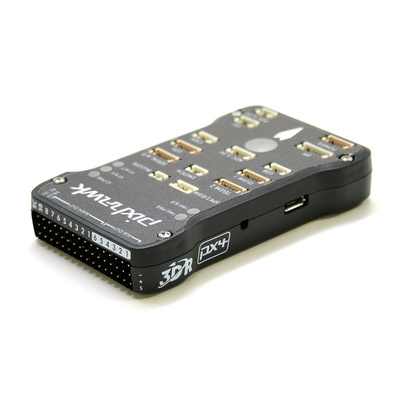
\includegraphics[width=0.35\textwidth]{pic/00_title/title.jpg}
	%\par\vspace{1cm}
	{\Large\itshape Pascal Häfliger\par}
	\vfill
	betreut durch:\par
	Prof.~Dr.~ Christoph \textsc{Eck}\par
	Prof.~Dr.~ Thierry \textsc{Prud'homme}\par
	\vspace{1cm}
	Industriepartner:\par
  Aeroscout GmbH, Horw\par
  %\textsc{Aeroscout GmbH, Horw}\par
  %\textsc{Aeroscout} GmbH, Horw\par


	

	\vfill  % Rest der Titelseite mit Leerraum auffüllen

% Bottom of the page
	{\large \today\par}
\end{titlepage}



\clearpage
\section*{Selbstständigkeitserklärung}

Hiermit erkläre ich, dass ich die vorliegende Arbeit selbstständig angefertigte und keine anderen als die angegebenen Hilfsmittel verwendet habe. Sämtliche verwendete Textausschnitte, Zitate oder Inhalte anderer Verfasser wurden ausdrücklich als solche gekennzeichnet.\\
\\
\\
\\
\noindent\rule{7cm}{0.4pt}   \rule{1cm}{0pt}  \rule{7cm}{0.4pt}\\
\noindent
Ort, Datum\rule{5.1cm}{0pt} \rule{1cm}{0pt}  Unterschrift
%$\overline{Datum, Ort\qquad \qquad} \qquad \overline{Unterschrift \qquad \qquad \qquad \qquad}$

\clearpage
\section*{Abstract}

Pixhawk is an embedded autopilot project with a tremendous market potential. This Product had just been upgraded to a new version. A flight controller has to run stable under any circumstances. Malfunctioning may cause severe damage to the aircraft and its surroundings. The main objective for this paper is to compare and implement a hardware in the loop test bench for such product. Utilizing this procedure, several test cases can be executed without the risk of damage. Also, a Simulink plugin was reviewed for stated requirements. However, that  expansion was unable to fulfill the specificaion and therefore not persued. Thus, a different approach was  evaluated. The source code for the Pixhawk firmware was altered to integrate a feasibility to access the internal data such as sensor values or actuating variables. Moreover, an enviroment simulation was designed with Matlab/Simulink to be run on a host PC. This paper offers a slim, expandable, reuasable hardware in the loop solution for Pixhawk. 

\clearpage


% Inhaltsverzeichniss
\tableofcontents
\clearpage


% Glossary
%\glsaddall
%\printglossary

\begin{multicols}{2}
	\glossarystyle{altlistgroup}
	\glsaddall
	\printglossary[title=Glossar]
\end{multicols}
\clearpage


%Einführung pixhawk & HIL
\section{Einführung}
\label{sec:Einführung}
Diese Arbeit handelt von einer bidirektionalen Datenstromrealisierung zwischen Simulink und einem embedded Board namens Pixhawk. Diese Daten sollen in einer Hardware in the Loop Simulation verwendet werden.\\

\noindent Im Kapitel \ref{sec:Was ist Pixhawk} und \ref{sec:Toolchains} werden die Grundlagen von Pixhawk sowie der Programmierumgebung erklärt und aufgezeigt. Weiter wird das Konzept der Hardware in the Loop Simulation an einigen Beispielen veranschaulicht, welches anschlissend mit dem Pilot Support Package versucht wurde zu realisieren.\\

\noindent Als Lösungskonzept der Hardware in the Loop Simulation wurde schlussendlich der Programmcode vom Pixhawk geändert. Auf der Gegenseite wurde im Simulink eine Datenstromverarbeitung und Simulation erstellt. Dieser Ansatz wird im Kapitel \ref{sec:App entwicklung} sowie \ref{sec:Simulink} aufgezeigt.



\subsection{Aufgabenstellung}

Bei der folgenden Aufgabenstellung handelt es sich um eine Kurzzusammenfassung. Die komplette Anforderungsliste ist in Kapitel \ref{sec:Anhang} ersichtlich.

\begin{itemize}
\item Einarbeitung in die Pixhawk Firmware und Designpatterns
\item Eigene Test-App mit Datenstromverarbeitung demonstrieren
\item Kommunikationsmöglichkeiten zwischen Pixhawk und Simulink ausarbeiten
\item Hardware in the Loop Simulation verwirklichen
\item Eigene App schreiben, welche die Komunikation mit Simulink übernimmt
\item Einfache Hardware in the Loop Simulation auf Seiten Simulink programmieren und demonstrieren.
\end{itemize}

\clearpage


\section{Was ist Pixhawk}
\label{sec:Was ist Pixhawk}

%\begin{wrapfigure}{r}{0.30\textwidth}
%  \vspace{-20pt}
%  \begin{center}
%    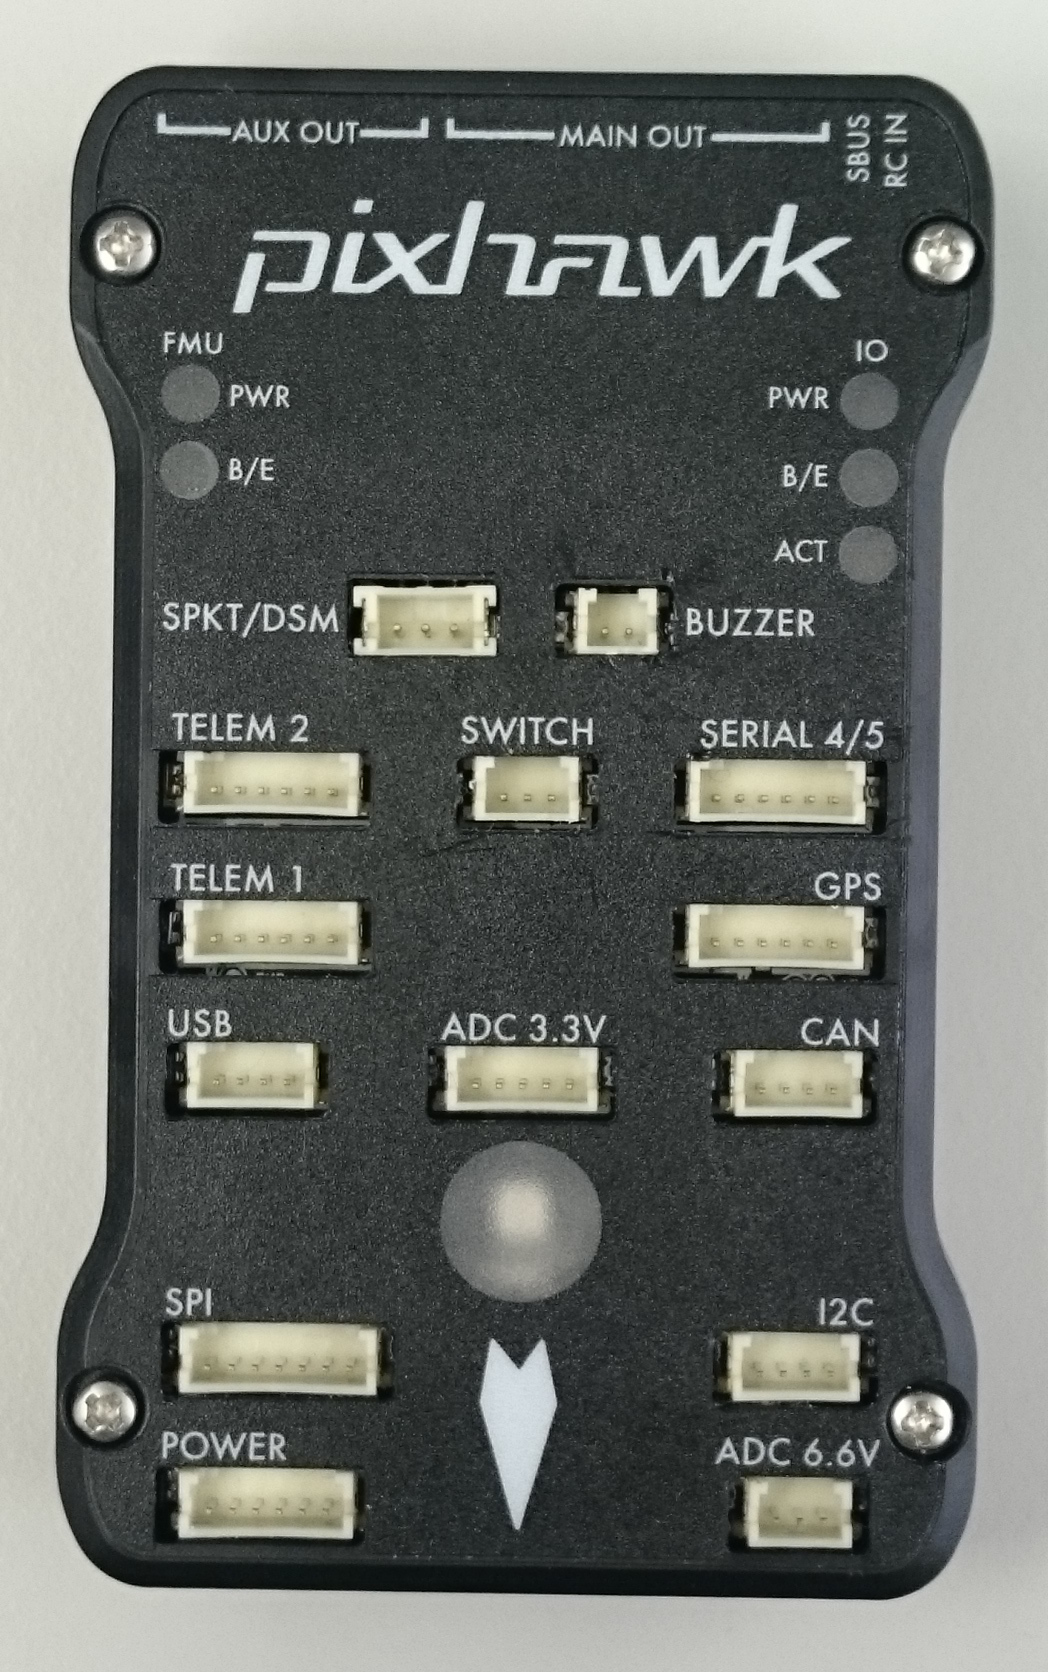
\includegraphics[width=0.28\textwidth]{pic/20_pixhawk/pixhawk_alone.jpg}
%  \end{center}
%  \vspace{-20pt}
%  \caption{Pixhawk}
%  \vspace{-10pt}
%\end{wrapfigure}


Das open-source Projekt Pixhawk ist ein Hochleistungsautopilot für Modellflugzeuge, Multicopter, Helikopter, Autos und Boote. Es wurde an der ETH Zürich entwickelt und ist nun auf dem Markt verfügbar. Das Pixhawk ist die zweite Version des Flugreglers. Für die Verwendung sowie Weiterentwicklung stehen zahlreiche Tools, Anleitungen und eine aktive Community zur Verfügung .\\
Für die Arbeit dient das Pixhawk zur Regelung eines Quadrocopters oder Modellhubschraubers.

\begin{figure}[ht]
  \begin{center}
  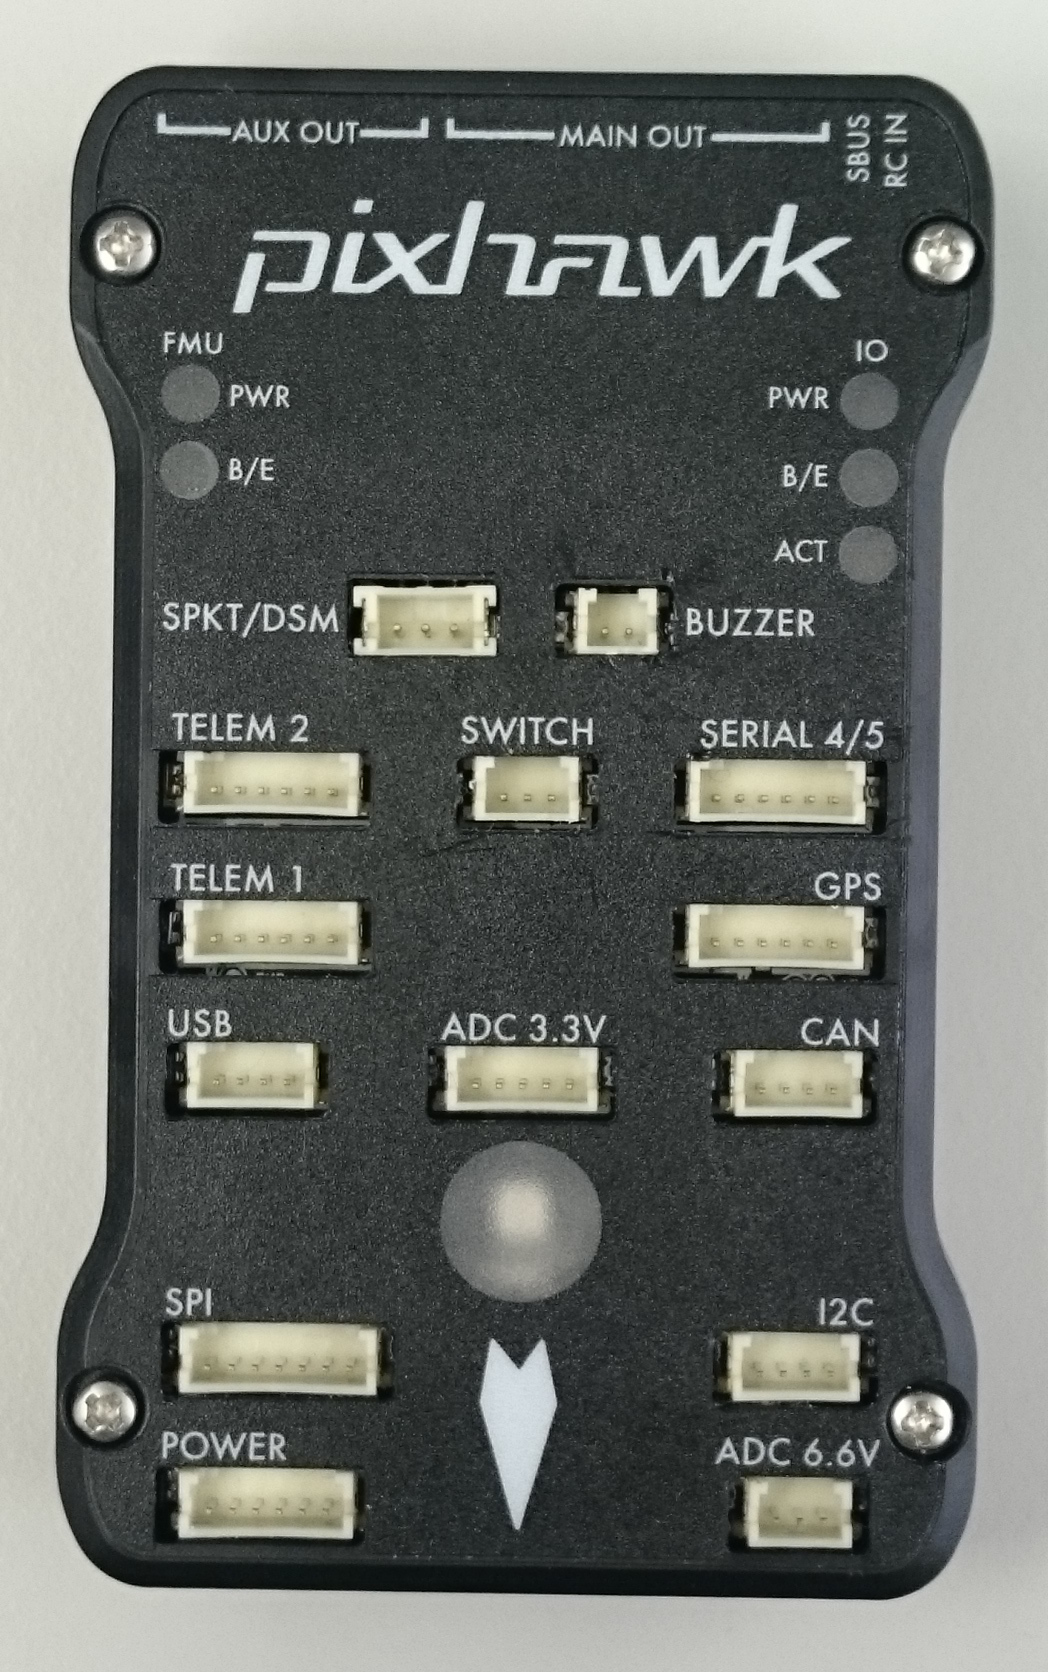
\includegraphics[width=0.3\textwidth]{pic/20_pixhawk/pixhawk_alone.jpg}
  \end{center}
  \caption{Pixhawk}
\end{figure}

Die wichtigsten Features des Pixhawks sind:
\begin{itemize}
\item 32-bit 168 MHz Cortex M4F (floating point unit)
\item 256 KB RAM, 2 MB Flash
\item MPU6000 als Accelerometer und Gyrometer
\item Power Controller mit Ausfallsicherung
\item ESC protection und überstrom Schutz
\item 5x UART, I2C, SPI, CAN, SD Karte, PWM, PPM, AD Wandler
\end{itemize}



\clearpage
%\input{tex/20_pixhawk/linux}
\subsection{POSIX}
POSIX (\acrlong{posix}) ist eine Erweiterung zum IEEE 1003, welche die API, Shell und Utilities von UNIX standartisierte.
Ursache für POSIX war, dass UNIX Software nicht auf allen UNIX Systemen lief.
Durch diese Standardisierung soll ein Skript oder Programm portierbar sein, ohne das eine Änderung im Sourcecode vorgenommen werden muss. Der Vorteil liegt darin, dass es auf jedem System läuft. Dadurch wird jedoch der technische Fortschritt stark abgebremst, weil es auch auf dem ältesten System laufen soll, welches z.B. ein 8 Bit Prozessor besitzt. Wenn man z.B. die Shell betrachtet, muss alles für \textit{sh}, der originalen Bourne Shell, kompatibel sein. \cite{shotts2012linux}



\begin{figure}[ht]
  \begin{center}
  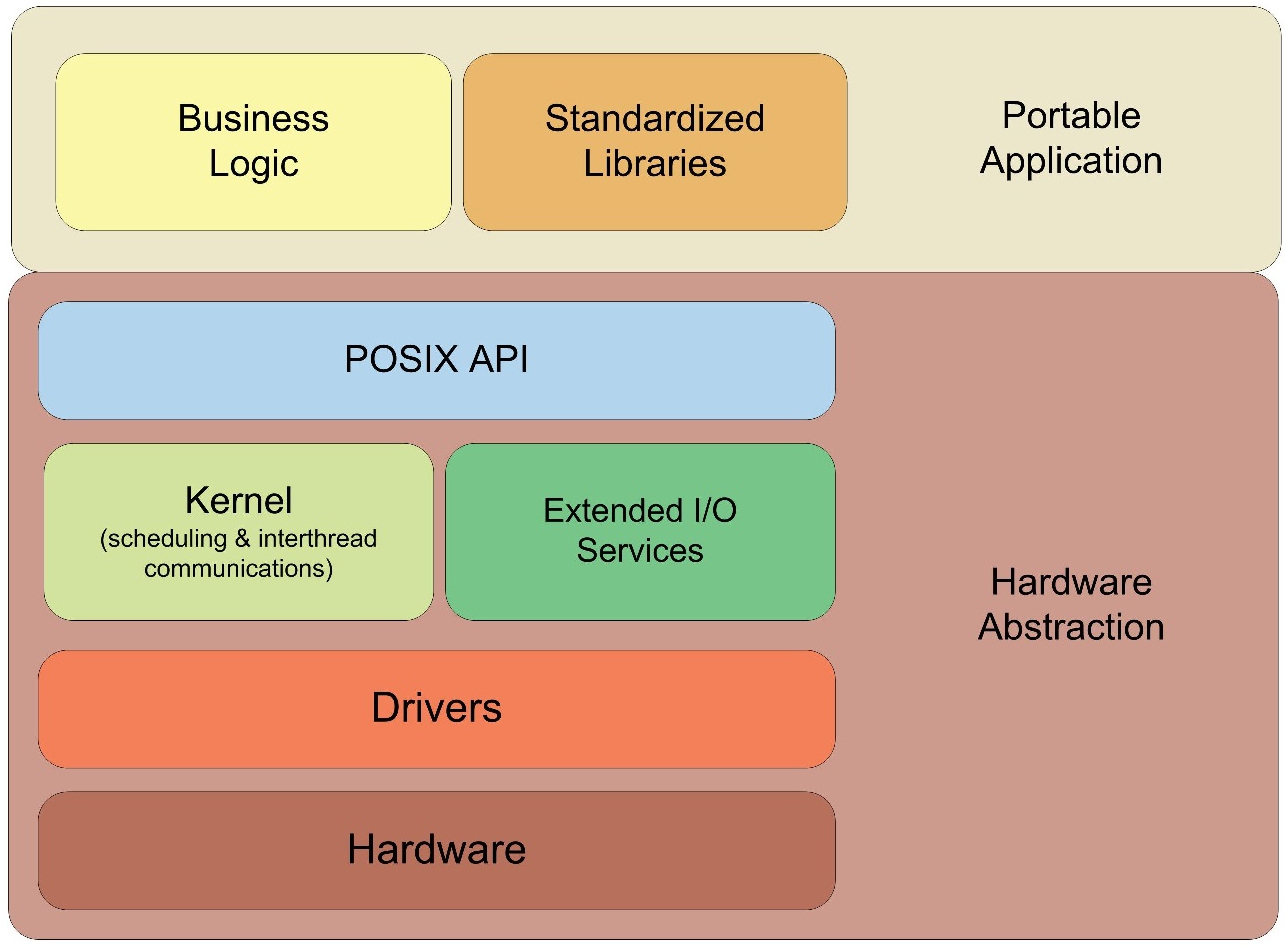
\includegraphics[width=0.48\textwidth]{pic/20_pixhawk/POSIX_RTOS_Model.jpg}
  \caption{POSIX API}
  \cite{posix_pic}
  \label{fig:posix}
  \end{center}
\end{figure}


\noindent In der Abbildung \ref{fig:posix} ist ersichtlich, wie die Applikation durch den POSIX Layer von der Hardware getrennt wird. Dieses POSIX API stellt einfache Interfaces zur Verfügung, welche im Kernel oder dem erweiterten I/O Service implementiert wurden. \\
Die Applikation kann nun auf jede Hardware portiert werden, da sie klar definierte Funktionen verwendet.

\clearpage
\subsection{Nuttx}
Nuttx ist ein RTOS (\acrlong{rtos}), welches auf 8 bis 32 Bit Architekturen läuft. Nuttx verwendet POSIX, damit das Operating System portierbar ist. Es ist open source, dadurch also hoch flexibel und anpassbar an die Bedürfnisse. Das Betriebssystem wird oft für kleine Embedded Systeme verwendet.
\\
Pixhawk verwendet Nuttx als Grundelement für ihre gesamte Struktur. Auf dem OS können dann mehrere Threads, sogenannte Apps, laufen. Diese verwenden das Preemtive Prinzip, also nicht kooperativ. Der Scheduler kümmert sich grösstenteils um die Einhaltung der Echtzeitkriterien.
\\
Der Cortex M4F besitzt nur 1 Kern, dadurch kann jeweils nur ein Thread laufen. Durch das Task switching können jedoch alle Tasks ihre Berechnungen durchführen. Der Scheduler, auch als Idel Task bekannt, gibt jedem Thread ein Zeitfenster, welches voll ausgenützt werden kann. Falls ein Task nicht das komplette Zeitfenster belegt, soll dieser die Ressourcen freigeben für andere Apps. Falls kein Thread Rechenzeit benötigt, wartet der Scheduler in einer Sleep ähnlichen Funktion. Im Hintergrund läuft dann der Garbage Collector und verwaltet die Speicherblöcke.\\
\\
Über eine UART (\acrlong{uart}) Schnittstelle kann man auf die nsh (\acrlong{nsh}) zugreiffen. Dies ermöglicht die Überwachung und Ausführung des Systems wie bei einem Terminal. Mit dem Befehlt top kann der Taskmanager angezeigt werden. Wie man aus der Abbildung \ref{fig:top} entnehmen kann, ist der Idel Task mit einer CPU Auslastung von 76\% stark vertreten. Die anderen Apps wie z.B. gps, px4io, sdlog2 laufen alle auch auf dem System.

\begin{figure}[ht]
  \begin{center}
  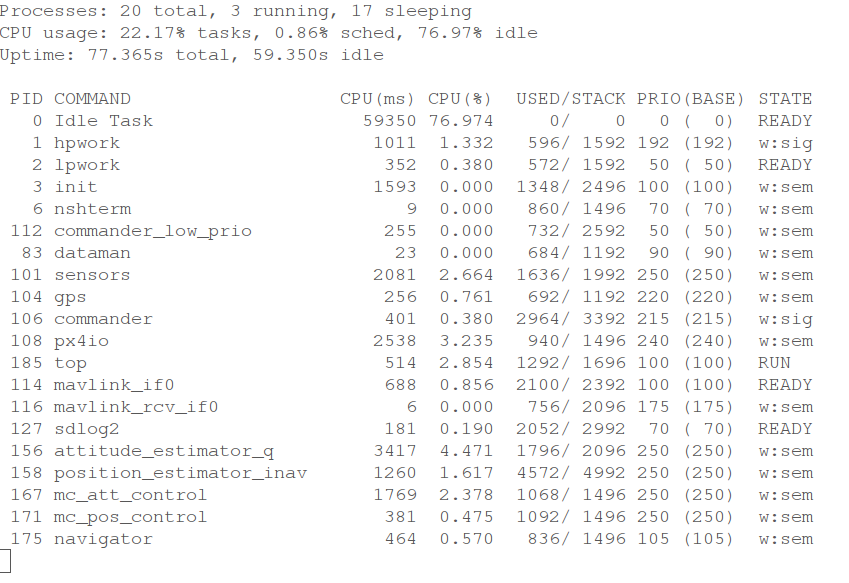
\includegraphics[scale=0.5]{pic/20_pixhawk/top2.png}
  \caption{Befehl top}
  \label{fig:top}
  \end{center}
\end{figure}

\clearpage
\subsection{uORB}

Die uORB (\acrlong{uorb}) wird auf dem Pixhawk verwendet um Datenstrukturen, sogenannte Topics, zwischen Apps, also Threads, auszutauschen. Dies ermöglicht eine ressourcenarme Möglichkeit, auf interne Daten zu warten per Betriebssystem Interrupt.
Man kann einen Filedescriptor auf ein gewünschte Topic anlegen, wie in folgendem Codebeispiel ersichtlich ist. 

\begin{lstlisting}
  //File descriptor erzeugen und zuweisen
	struct sensor_combined_s raw;
	int sensor_sub_fd = orb_subscribe(ORB_ID(sensor_combined));
	struct pollfd fds_uorb[]= {
		{ .fd = sensor_sub_fd,   .events = POLLIN },
	};
	
    [...]
  
	//Warte auf neue Daten per OS Interrupt
	poll_ret = poll(fds_uorb, 1, TIMEOUT_MS);
	
	if (poll_ret <= 0)
	  //Keine Daten erhalten
	else
	  //Neue Daten erhalten

\end{lstlisting}

%\caption{Thema abonnieren und auf Daten warten}

\noindent
Hier wird ein Filedescriptor erzeugt, welcher alle Sensordaten abonniert. Falls während dem Timeout 'TIMEOUT\_MS' neue Daten auf die uORB geschrieben wurden, wird ein Interrupt ausgelöst und der return Wert wird grösser 0 sein.


\subsection{cmake}
Die Applikationsentwicklung auf dem Pixhawk ist modular aufgebaut. Durch Verwendung von cmake können Kompilerparameter einfach geändert oder Codesegmente hinzugefügt werden. Pixhawk führte cmake gegen Ende 2015 neu ein. Vorher basierte der Build Prozess auf make.

\noindent Durch folgende \textit{CMakeLists.txt} Datei werden zwei neue Sourcedateien namens \textit{my\_app.c} und \textit{crc.c} zum Build Prozess hinzugefügt. Die Priorität wurde sehr hoch angesetzt. Der Stack liegt mit 1200 Bytes auf der sicheren Seite. Stackoverflows sollten dadurch nicht vorkommen, solange keine rekursiven Methoden verwendet werden.\\
\noindent Falls die App programmiert wurde, kann ihre main Methode mit dem Kommando my\_app in der nsh gestartet werden. Dies ist auf Zeile 3 definiert.

\begin{lstlisting}
px4_add_module(
	MODULE modules__my_app
	MAIN my_app
	PRIORITY "SCHED_PRIORITY_MAX-30"
	STACK 1200
	COMPILE_FLAGS
		#${MODULE_CFLAGS}
		#-Os
	SRCS
		my_app.c
		crc.c
	DEPENDS
		#platforms__common	)
\end{lstlisting}

\clearpage



%Programmierumgebung
\section{Toolchains}
\label{sec:Toolchains}
\subsection{Installation}
\begin{flushleft}

Die Installation der Pixhawk Toolchain wird auf \href{https://pixhawk.org/dev/quickstart}{www.pixhawk.org/dev/quickstart} für alle Betriebssysteme sehr detailliert und ausführlich erklärt.

\end{flushleft}



\subsection{Verwendung}
\noindent
Mit dem Kommando \textbf{make px4fmu-v2\_default} wird die Firmware kompiliert und die .elf Datei erzeugt. Mit \textbf{make px4fmu-v2\_default upload} wird die Firmware kompiliert, .elf Datei erzeugt, auf das Pixhawk per USB hochgeladen und dort programmiert.

\subsubsection{Linux}

Für Linux Benützer ist es zu empfehlen, ein alias für die Kommandos zu erstellen. Dies kann erzeugt werden durch:
\begin{lstlisting}
cd ~
vim .bashrc
\end{lstlisting}

\noindent
Anschliessend die Taste 'a' drücken für den Eingabe Modus. Jetzt folgende Zeilen eingeben:

\begin{lstlisting}
mk () {
  cd ~/path/to/Firmware/
  make px4fmu-v2_default
}

mkup () {
  cd ~/path/to/Firmware/
  make px4fmu-v2_default upload
}
\end{lstlisting}

\noindent
Der Pfad zur Firmware muss vorher angepasst werden. Durch ESC kann anschliessend in den Navigationsmodus gewechselt werden. Mit ':wq' werden die Änderungen gespeichert und das Programm verlassen. Der Pfad zur Firmware muss vorher angepasst werden. Zum Schluss muss die  \textbf{.bashrc} Datei neu kompiliert werden mit:

\begin{lstlisting}
source .bashrc
\end{lstlisting}

\noindent
Nun kann über das Terminal die Firmware kompiliert und hochgeladen werden mit dem Befehl 'mkup'. Falls man diesen nicht immer neu eingeben möchte, kann mit der Pfeiltaste $\uparrow$  oder !! das letzte Kommando erneut ausgeführt werden.\\

\noindent
Für die Programmierung empfiehlt sich die IDE Code::Blocks. Auch hierzu gibt es eine Anleitung unter \href{https://pixhawk.ethz.ch/toolchain/codeblocks}{https://pixhawk.ethz.ch/toolchain/codeblocks}. In der Anleitung sollten jedoch nur die stable builds verwendet werden und keine nightly builds.


\subsection{Troubelshooting}
Während der Arbeit mit dem Pixhawk traten keine Fehler auf. Das px4 v1 (Pixhawk Version1) hatte im Vergleich einige zeitkritische Probleme beim Löschen und Programmieren der Firmware. 
\clearpage



%Hardware-in-Loop
\section{Hardware in the Loop}
\label{sec:Hardware in the Loop}
\subsection{Einleitung}

Bei HiL (\acrlong{hil}) handelt es sich um eine Simulation, bei welcher die Sensoren und Aktuatoren des Systems getestet werden sollen. Diese Simulationen werden oft für eingebettet Systeme verwendet. Der Vorteil liegt darin, dass bei einem Modellabsturz keine Schäden entstehen und der Vorgang zu diesem Ereignis klar verfolgbar ist durch die Log Dateien.

\begin{figure}[ht]
	\begin{center}
		\begin{subfigure}{0.49\textwidth}
			\begin{center}
		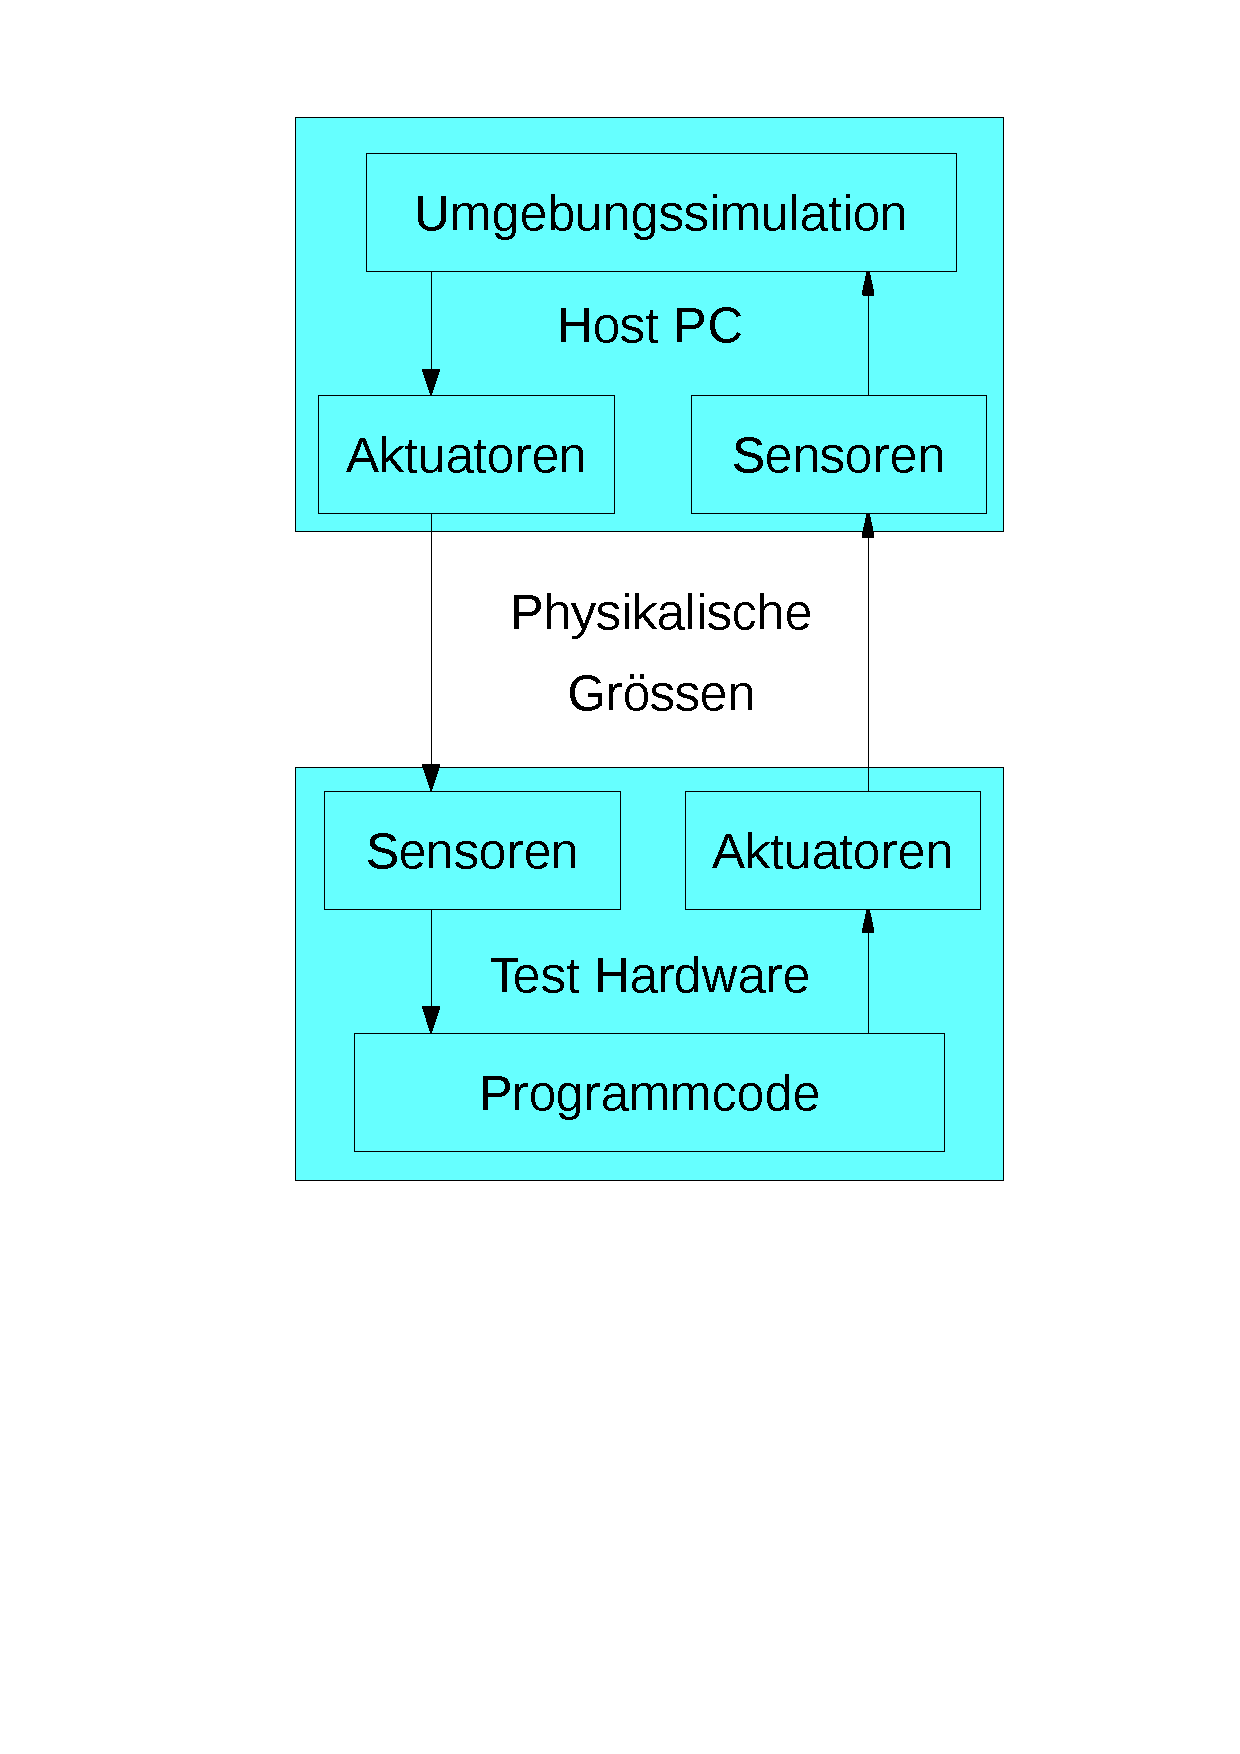
\includegraphics[height=0.33\paperheight, trim={5cm 9.5cm 4cm 2cm},clip]{pic/35_hil/hil_1.pdf} 
		\caption{Allgemeiner Hil Aufbau}
		\label{fig:hil_normal}
		\end{center}
		\end{subfigure}
		\begin{subfigure}{0.49\textwidth}
		\begin{center}
		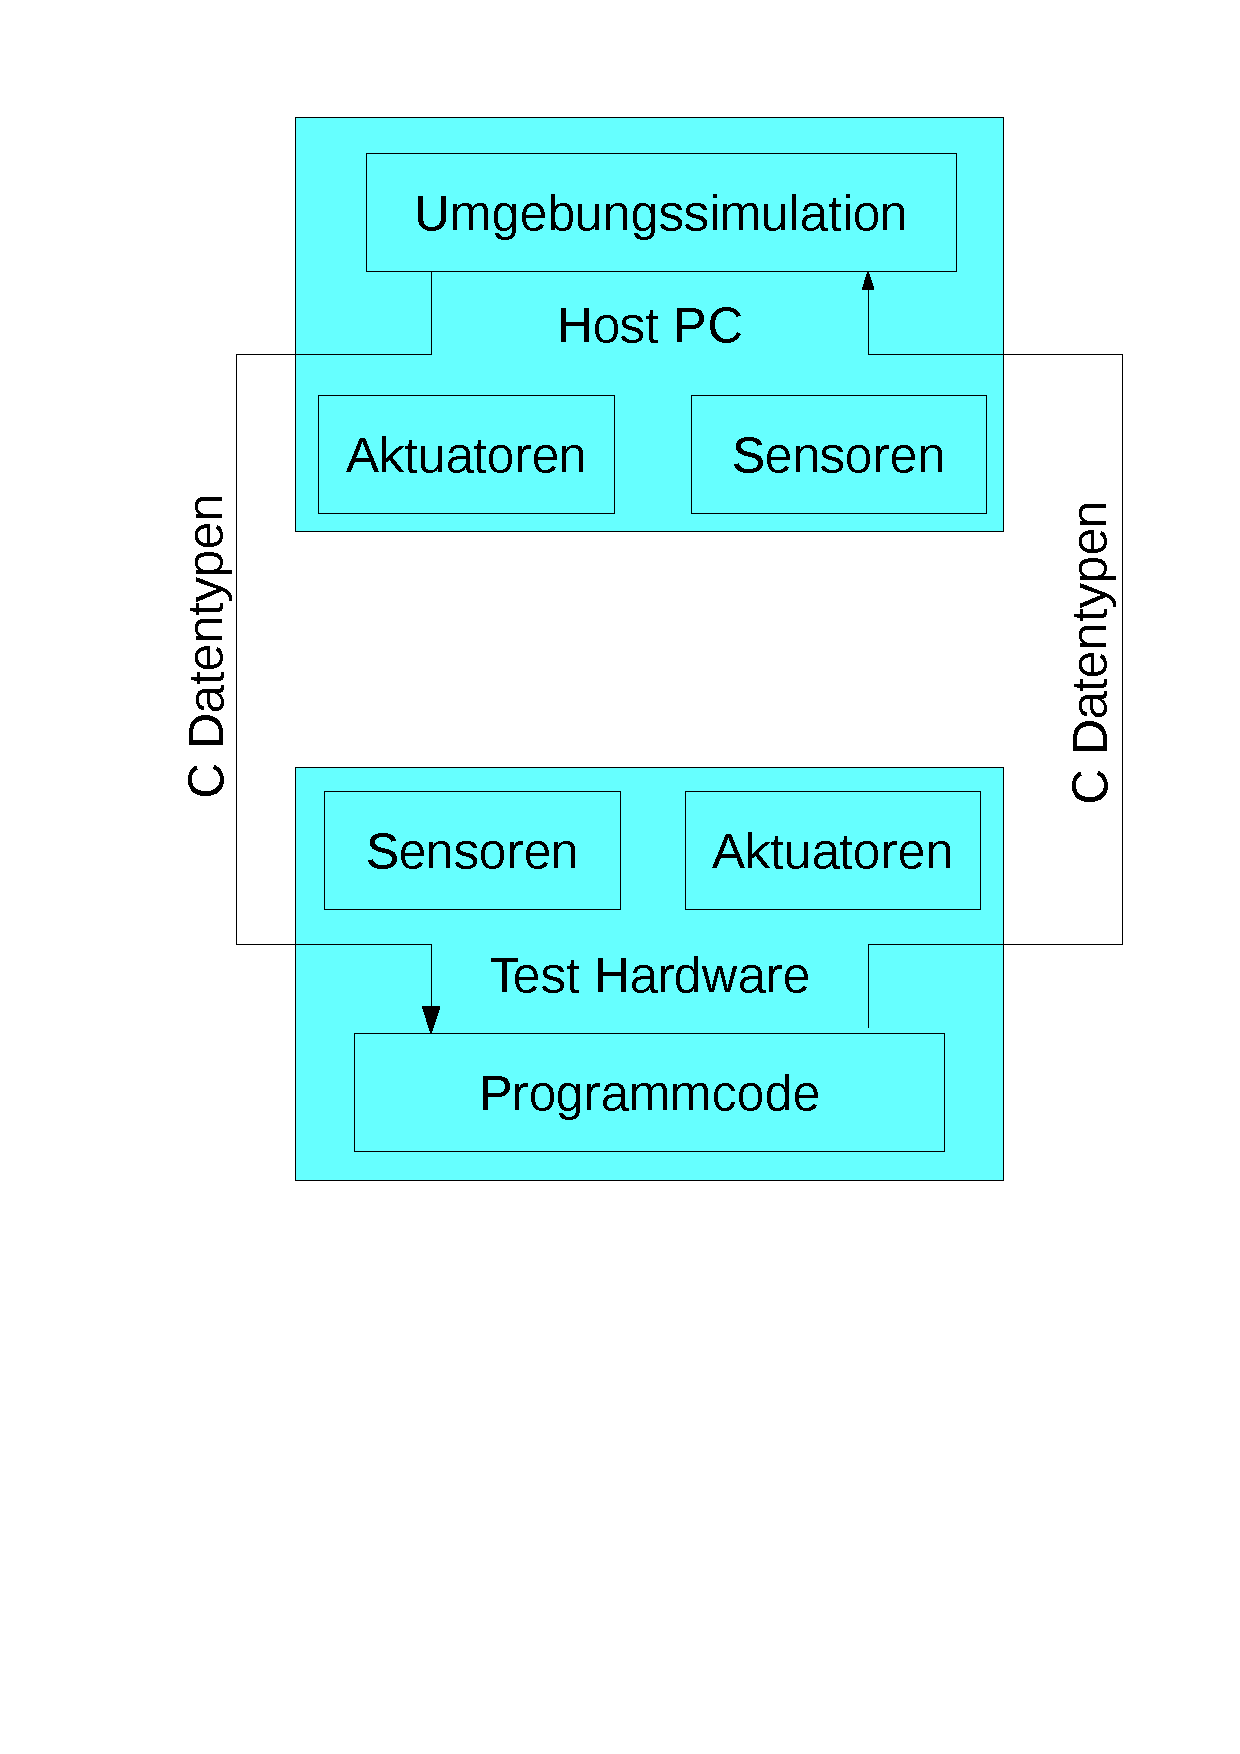
\includegraphics[height=0.33\paperheight, trim={3cm 9.5cm 1.5cm 2cm},clip]{pic/35_hil/hil_2.pdf}
		\caption{Pixhawk Hil Aufbau}
		\label{fig:hil_pixhawk}
		\end{center}
		\end{subfigure}
		\caption{Vergleich Hil Aufbau}
		\label{fig:hil_vergleich}
	\end{center}
\end{figure}

\noindent
Für die Pixhawk Simulation (Abbildung: \ref{fig:hil_pixhawk}) werden die elektrischen Signale abgegriffen, welche die Aktuatoren ansteuern würden. Dies senkt die Simulationskomplexität stark. Bei einer echten HiL Simulation (Abbildung: \ref{fig:hil_normal}) müssten die Aktuatoren und Sensoren der Test Hardware auch miteinbezogen werden.\\\\
Beispiel Rotoren:\\
Bei einer echten HiL Simulation würde der Rotorenschub der Test Hardware durch ein Anemometer gemessen. Dieses Signal würde dann in dem Umgebungssimulator ausgewertet und die Aktuatoren Stellgrössen berechnen.\\
Bei der Pixhawk HiL Simulation wird das PWM der Frequenzumrichter direkt an den Host PC per UART übermittelt. Die Aktautoren und Sensoren werden jeweils überbrückt.

\clearpage
\subsection{Pixhawk and HiL}
\label{sec:Pixhawk_and_HiL}


\subsubsection{Sensorrauschen und Kalmann Filter}
Hierbei handelt es sich \textbf{nicht} um eine HiL Simulation, sondern um einen ersten, einfachen Testaufbau mit funktionierender Datenübertragung zwischen Pixhawk und Simulink als Host PC. 

\begin{figure}[ht]
  \begin{center}
  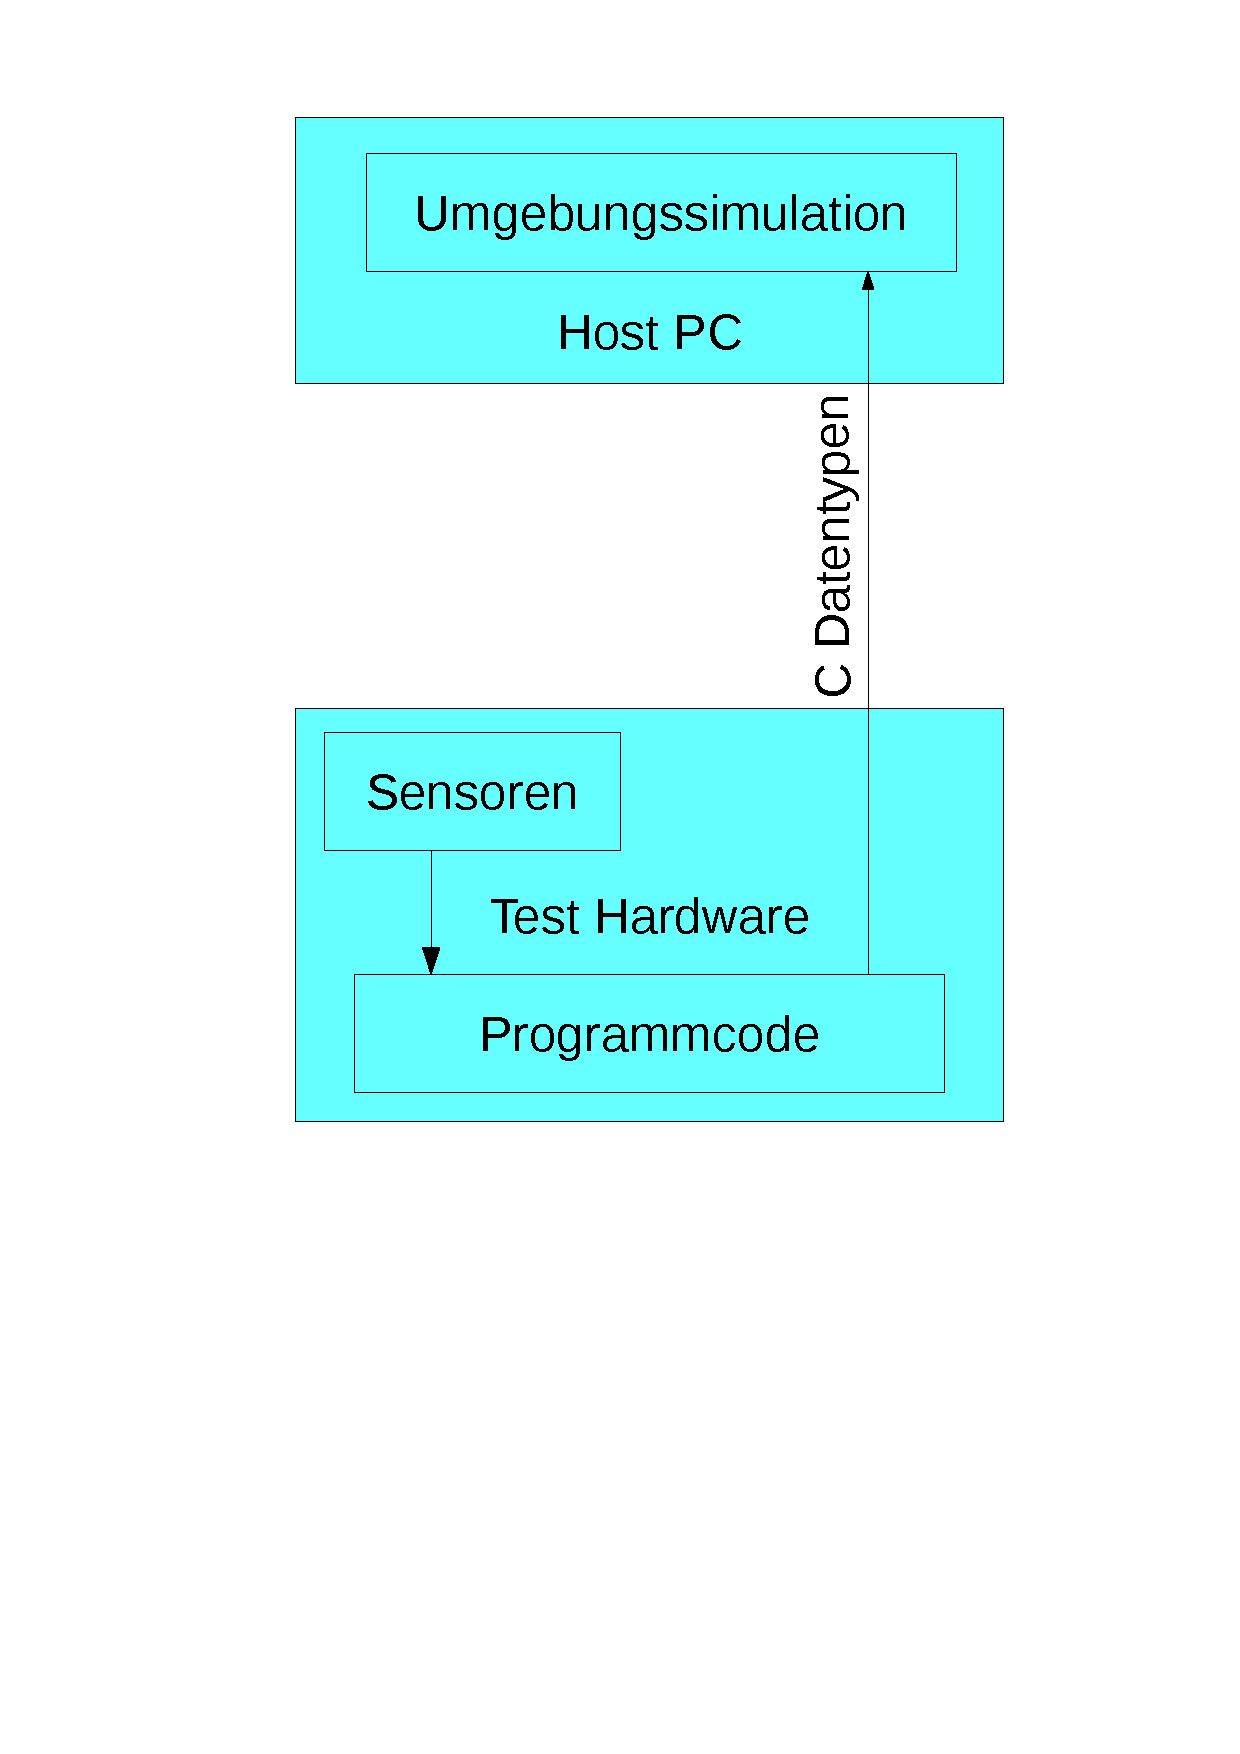
\includegraphics[scale=0.5, trim={5cm 10.6cm 2.5cm 2cm},clip]{pic/35_hil/hil_sensor_noise.pdf}
  \caption{Messung Sensorrauschen}
  \label{fig:messung_sensorrauschen}
  \end{center}
\end{figure}

\noindent Die Sensordaten wie Gyro-, Accelero-, Barometer und Temperaturfühler werden von der Test Hardware entgegengenommen. Diese Daten durchlaufen einen Kalmann Filter und liegen dann als roh-, sowie gefilterte Werte auf der uORB zur Weiterverarbeitung. Diese Werte werden dann im Programmcode abgegriffen und über eine serielle Schnittstelle an den Host PC übermittelt.\\
Auf dem Umgebungssimulator kann nun ein Kalmann Filter auf die roh Werte angewendet werden und mit den gefilterten Werten verglichen.



\subsubsection{Systemtest 1}
In einem weiteren Test könnte die Flugsteuerung vom Pixhawk getestet werden wie in Abbildung \ref{fig:hil_pixhawk} aufgezeigt. Die Datenübertragung wäre weiterhin auf einer seriellen Schnittstelle. Daruch wäre eine komplette HiL Simulation möglich.

\subsubsection{Systemtest 2}
Eine weitere Möglichkeit wäre, vorhandene Sensorwerte eines aufgezeichneten Flugs in the uORB einzuspeisen. Die berechnete Rotorenstellgrösse vom Pixhawk könnte man anschliessend mit den vorhandenen Aktuatorenwerten vergleichen.
\clearpage



%Matlab+Simulink PSP
\section{Pilot Support Package}
\label{sec:Pilot Support Package}
\subsection{Einführung}
Das PSP (\acrlong{psp}) ist eine offizielle Toolbox von MathWorks. Diese Erweiterung für Simulink und Pixhawk Firmware ermöglicht es, eigene Flugregler für Pixhawk in Simulink zu entwerfen, welche in Echtzeit auf dem Pixhawk laufen. Um dies zu realisieren, wurden neue Simulink Blöcke hinzufügt (siehe Abbildung \ref{fig:psp_all_blocks}). Diese Blöcke können entweder Sensordaten ausgeben oder Aktuatorendaten empfangen. \\
In Simulink kann die eigene Flugsteuerung als Blockschaltbild aufgebaut werden. Diese wird dann mit dem Code Composer als C Code generiert und in die Pixhawk Firmware eingebunden. 
 
\noindent Für die Verwendung muss zuerst die Toolbox unter  \href{https://ch.mathworks.com/hardware-support/forms/pixhawk-downloads.html}{https://ch.mathworks.com/hardware-support/forms/pixhawk-downloads.html} heruntergeladen werden. Auf derselben Seite steht eine Anleitung mit Beispielen zur Verfügung.

\begin{figure}[ht]
  \begin{center}
  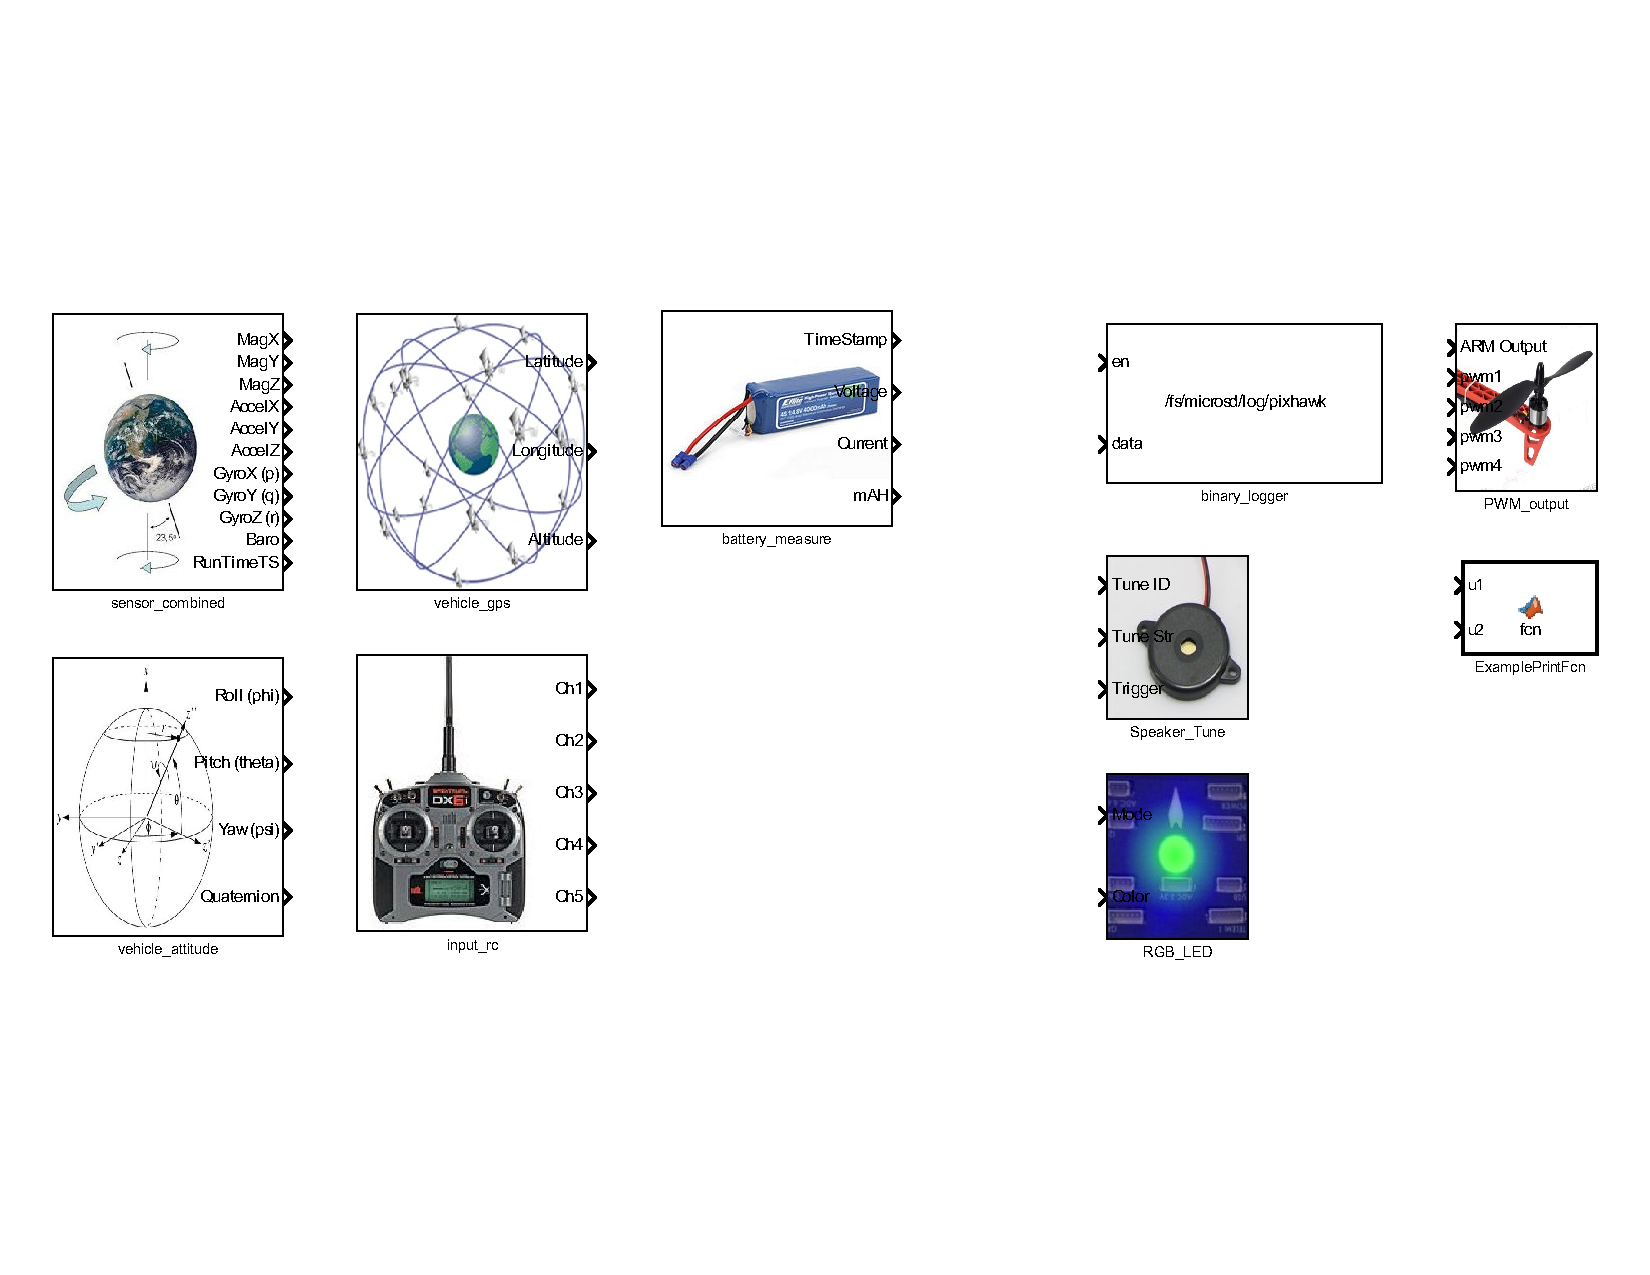
\includegraphics[scale=0.5, trim={0.5cm 5cm 0.5cm 5cm},clip]{pic/40_psp/all_blocks.pdf}
  \caption{PSP Blöcke}
  \label{fig:psp_all_blocks}
  \end{center}
\end{figure}

%MathWorks stellt eine Erweiterung für Pixhawk zur Verfügung. Dieses PSP \acrlong{psp}  ermöglicht die Simulation der FCS \acrlong{fcs} und kann daraus C-Code generieren, welcher anschlissend als App auf dem Pixhawk läuft. 

\cite{mathworks_psp}

\subsection*{Installation}
Die Installationsdateien sowie Dokumentation können hier bezogen werden. Das Benutzerhandbuch erklärt den gesammten Installationsprozess.\\
\href{ch.mathworks.com/hardware-support/forms/pixhawk-downloads.html}{ch.mathworks.com/hardware-support/forms/pixhawk-downloads.html}\\
\href{ch.mathworks.com/hardware-support/files/Simulink_Pixhawk_Support.pdf}{ch.mathworks.com/hardware-support/files/Simulink\_Pixhawk\_Support.pdf}


\begin{quote}
"PX4 Software Download [...] This download script has been modified in the PSP installer to download from a Github repository containing a forked stable copy of the PX4 FMU firmware. This stable-release will be revisited from time to time by MathWorks Pilot Engineering to ensure appropriate updates are applied from the official firmware when necessary (ie: bug fixes, feature updates). Please contact us regarding any discrepancies between the forked and the official repo."\cite{mathworks_psp}
\end{quote}
\begin{flushleft}
Durch die Installation des Packages wird nicht mehr der offizielle Realease von Pixhawk verwendet, sondern ein unbekannt datierter Branch von MathWorks.Somit werden Bugfixes oder neue Features erst verspätet im MathWorks Branch zu verwenden sein.
\end{flushleft}


\subsection{Ausführung}
Für die Ausführung und Verwendung der Simulink Modelle sollte vorzugsweise die PSP Anleitung konsultiert werden. Auf mehreren Seiten ist der Vorgang sowie Projekteinstellungen detailliert und ausführlich erklärt.\\
Anbei wird eine Flugregelung erzeugt, welche auf dem Pixhawk läuft und über das Simulink gesteuert werden kann. Das Vorgehen basiert auf den folgenden Schritten:\\

\noindent
\textbf{Modellentwurf}\\
Das Modell in Abbildung \ref{fig:psp_modell} enthält den Flugregler, welcher später auf dem Pixhawk laufen soll. Der Regler berechnet anhand den Sensordaten die Stellgrössen der Aktuatoren.
\begin{figure}[H]
  \begin{center}
  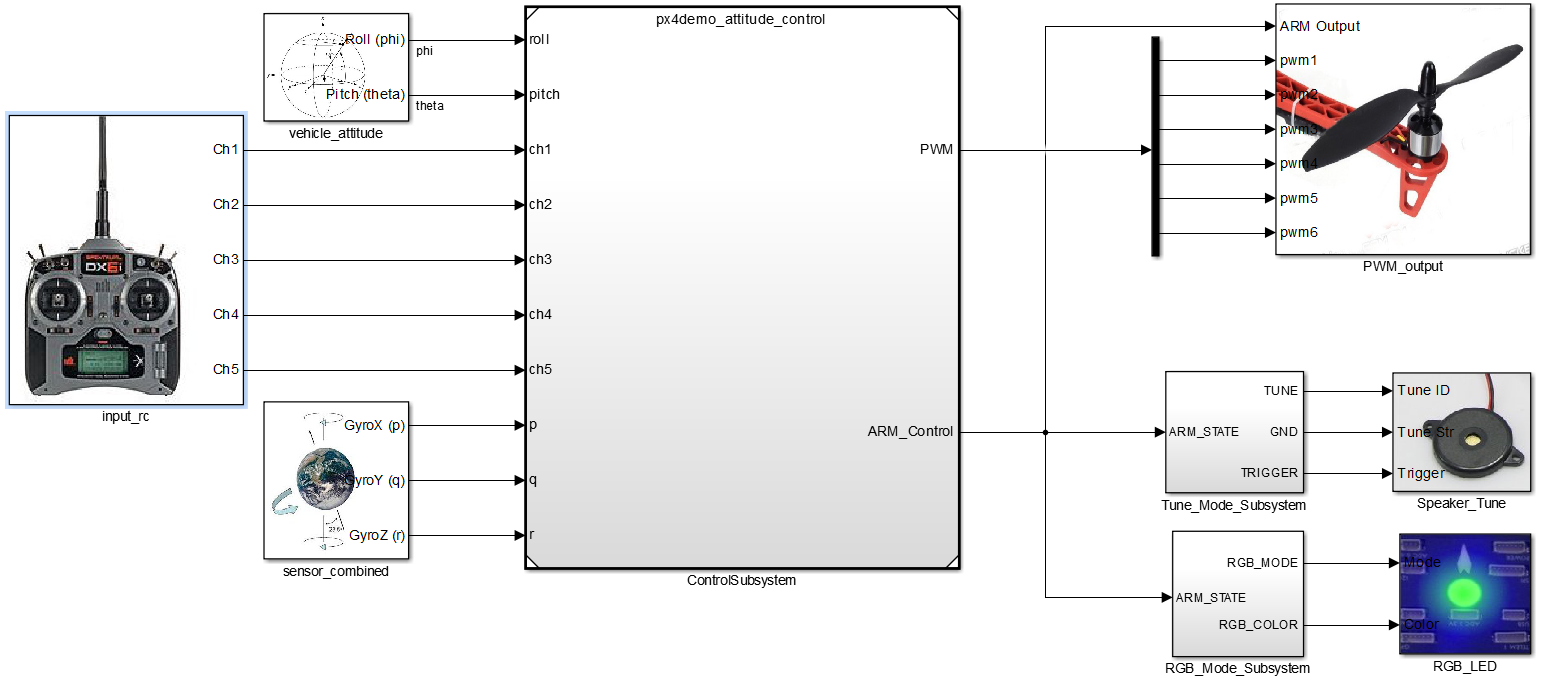
\includegraphics[scale=0.3]{pic/40_psp/psp_model.png}
  \caption{Simulink Modell}
  \label{fig:psp_modell}
  \end{center}
\end{figure}

\noindent
\textbf{Projekteinstellungen}\\
Eine Vielzahl von Einstellungen muss für den Code Composer vorgenommen werden. Je nach Verwendungszweck weichen diese ab.

\begin{figure}[H]
  \begin{center}
  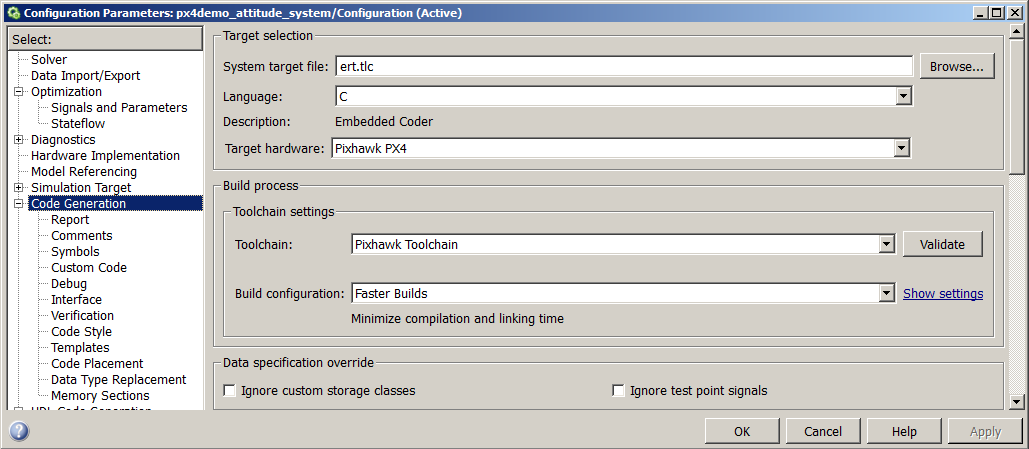
\includegraphics[scale=0.3]{pic/40_psp/psp_settings.png}
  \caption{Projekteinstellungen}
  \label{fig:psp_config}
  \end{center}
\end{figure}

\noindent
\textbf{Codegeneration}\\
Durch bestätigen des Knopfs in Abbildung \ref{fig:psp_generate} wird aus dem Simulink Blockschaltbild lauffähigen C Code generiert. Dieser Programmcode enthält mehrere Apps, welche automatisch auf das Pixhawk geladen werden. In Abbildung \ref{fig:psp_diagnostic} ist der Simulink Diagnostic Viewer ersichtlich. Hier wird aufgezeigt, dass der C Code erfolgreich zu einer .elf Datei kompiliert wurde und auf das Pixhawk geladen würde.

\begin{figure}[H]
  \begin{center}
  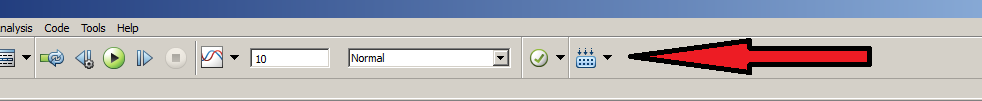
\includegraphics[scale=0.3]{pic/40_psp/psp_generate.png}
  \caption{Code generieren und hochladen}
  \label{fig:psp_generate}
  \end{center}
\end{figure}

\begin{figure}[H]
  \begin{center}
  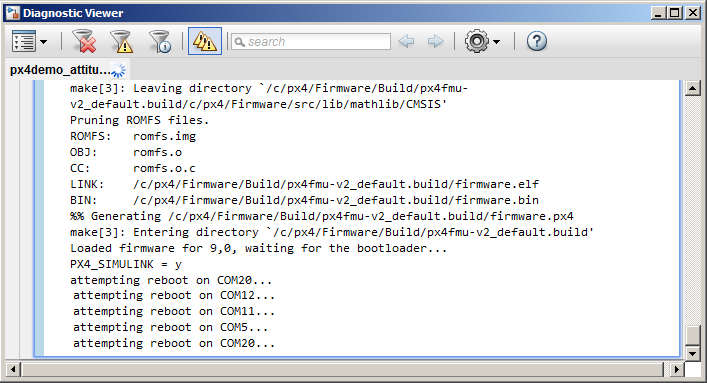
\includegraphics[scale=0.3]{pic/40_psp/psp_upload.png}
  \caption{Diagnostic Viewer}
  \label{fig:psp_diagnostic}
  \end{center}
\end{figure}


\noindent
\textbf{Simulation / realer Test}\\
Der Flugregler aus Abbildung \ref{fig:psp_modell} ist nun auf dem Pixhawk implementiert. Das Modell kann auf zwei Arten gestartet werden:
\begin{itemize}
\item Durch den 'run' Knopf im Simulink
\item Mit dem nsh Kommando px4\_simulink\_app start
\end{itemize}

\medskip


\subsection{Auswertung}
Das PSP dient dazu eigene Flugregler mit einfachen Mitteln und ohne Programmierkenntnissen zu entwerfen, realisieren und auf dem Fluggerät in realer Umgebung zu testen.

\noindent Weiter können Parameter (z.B. P-, I- Anteil, Matritzen) während der Laufzeit geändert werden. Dies sollte jedoch aufgrund der Performance nicht während dem Flug vorgenommen werden.\\

\noindent Im Simulink Modell können auch die Signale der PSP Blöcke zur Laufzeit angezeigt werden. Dadurch hat man einen Überblick der Gyro- Accel-, Batterie-Werte. Dies ist jedoch nur während der kabelgebundenen Ausführung möglich.
\\

\noindent Das Tool hat jedoch nicht nur Vorteile. Durch die Struktur der Blöcke ist \textbf{keine} HiL Simulation, wie in Abbildung \ref{fig:hil_pixhawk} aufgezeigt, möglich. Für die Umgebungssimulation auf Seiten Simulink (Host PC) stehen nur die Sensorenwerte zur Verfügung und nicht jene der Aktuatoren. Dadurch findet der Kreislauf in reversierter Abfolge statt.\\

\noindent Als weiterer Negativpunkt sind umständlichen Projekteinstellungen in Simulink aufzuführen. Diese weichen in jedem Beispielprojekt voneinander ab und falls ein Häcken bei einer Option falsch gesetzt wurde, funktioniert der Code Composer nicht. Die Fehlerausgabe dieses Tool ist dann bei der Fehlersuche nicht hilfreich.
 
\clearpage


%Programmierung
\section{Eigene HiL Simulation Entwicklung}
Aufgrund des Misserfolgs vom PSP, wurde ein neuer Weg eingeschlagen. Es gibt bereits fertige, komplexe Pixhawk HiL Simulatoren, jedoch basieren diese auf mehreren, teils kostenpflichtigen, Programmen und der Support für diese Applikationen ist nicht gewährleistet.\\
Deshalb wurde eine eigene App für das Pixhawk entwickelt, welche die Daten auf dem Mikroprozessor modifizieren, auslesen oder einfügen kann. Dadurch ist dieses Lösungskonzept sehr mächtig, offen und erweiterbar. Auf der Gegenseite wurde eine Umgebungssimulation in Simulink programmiert, welche ohne Verzögerung ihre Aufgabe erfüllen soll.


\subsection{App Entwicklung}
\label{sec:App entwicklung}
Dieses Kapitel beschreibt der Aufbau der Pixhawk App. Dieses Programm kann völlig losgelöst vom Simulink programmiert werden.


\subsubsection{Statemachine}
Für diese App wurden mehrere Statemachines eingesetzt. Eine übernimmt die komplette Businesslogik für den Ablauf des Programms. Eine zweite Statemachine sorgt dafür, dass die serielle Datenkommunikation korrekt interpretiert wird.


\paragraph{Businesslogik}\mbox{}\\
Die App besitzt zwei Threads. Der Erste ist nur für die Kommunikation und Interpretation der nsh Kommandos verantwortlich. Dieser Thread läuft nur ein paar Zyklen lang und steuert den zweiten Task. Die Steuerkommandos sind start, stop, status, help.\\

\noindent Der zweite Thread übernimmt die gesammte Businesslogik, welche in Abbildung \ref{fig:Statemachine Businesslogik} aufgezeigt wird. In dieser Logik werden jeweils Daten zwischen Interfaces ausgetauscht.\\

\begin{figure}[ht]
  \begin{center}
  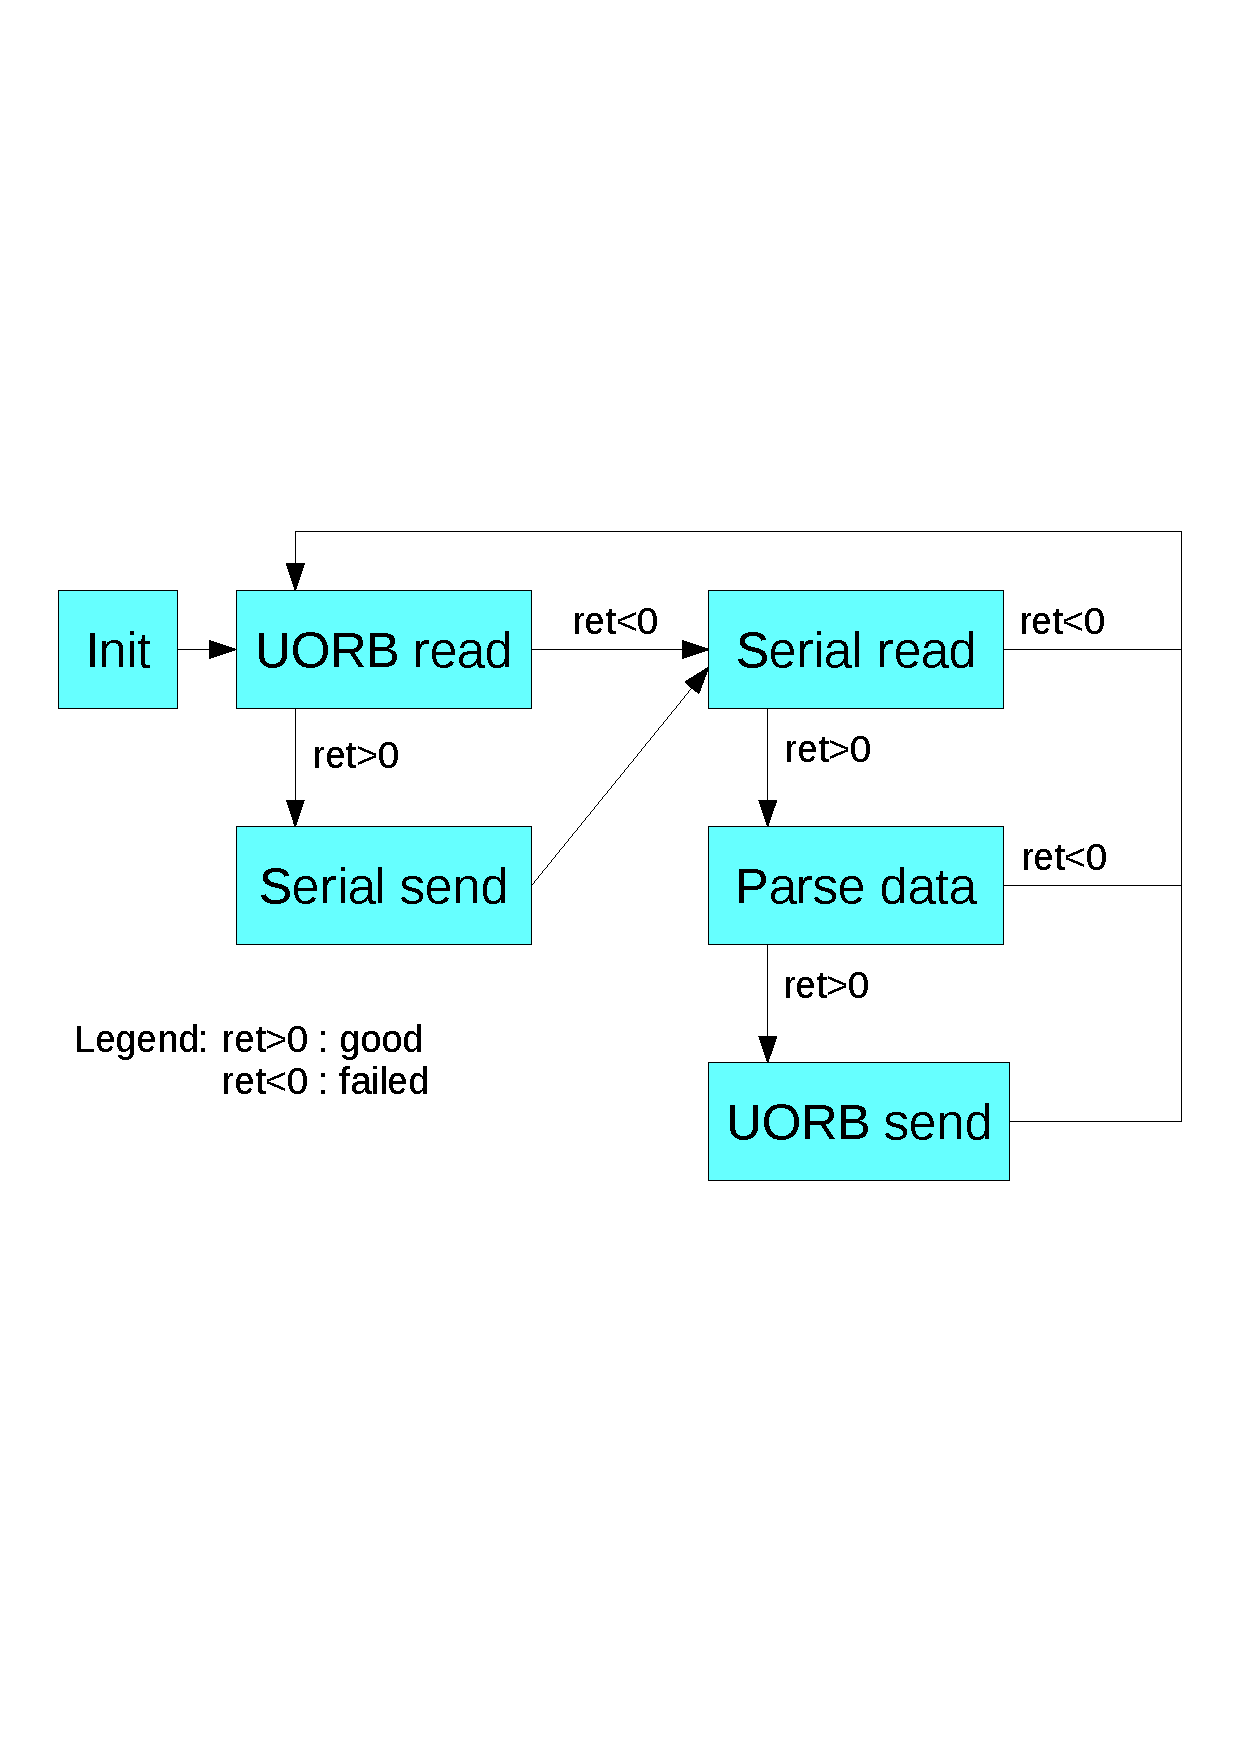
\includegraphics[scale=0.5, trim={1cm 9.5cm 0cm 9cm},clip]{pic/50_app/statemachine_thread.pdf}
  \caption{Statemachine Businesslogik}
  \label{fig:Statemachine Businesslogik}
  \end{center}
\end{figure}

\noindent Nach der Initialisierung werden zwei 2 Hauptaufgaben ausgeführt. Zum einen die uORB Pakete auf die UART übertragen, zum anderen die UART Pakete in die uORB weiterleiten. Dieses Vorgehen ist in obiger Abbildung detailliert erklärt. Die Zustandsfunktionen haben jeweils einen return Wert (ret). Anhand dieses Wertes wird jeweils das weitere Vorgehen bestummen.

\clearpage
\paragraph{Parser}\mbox{}\\

\noindent Die Daten werden jeweils als Paket übertragen. Diese Struktur ist in Abbildung \ref{fig:packet1} aufgezeigt. Eine Erweiterung wäre die ID der Payload zu übermitteln. Dadurch wüsste man, um welches uORB Topic es sich handelt.

\begin{figure}[ht]
	\begin{center}
		\begin{subfigure}{0.49\textwidth}
%			\begin{center}
		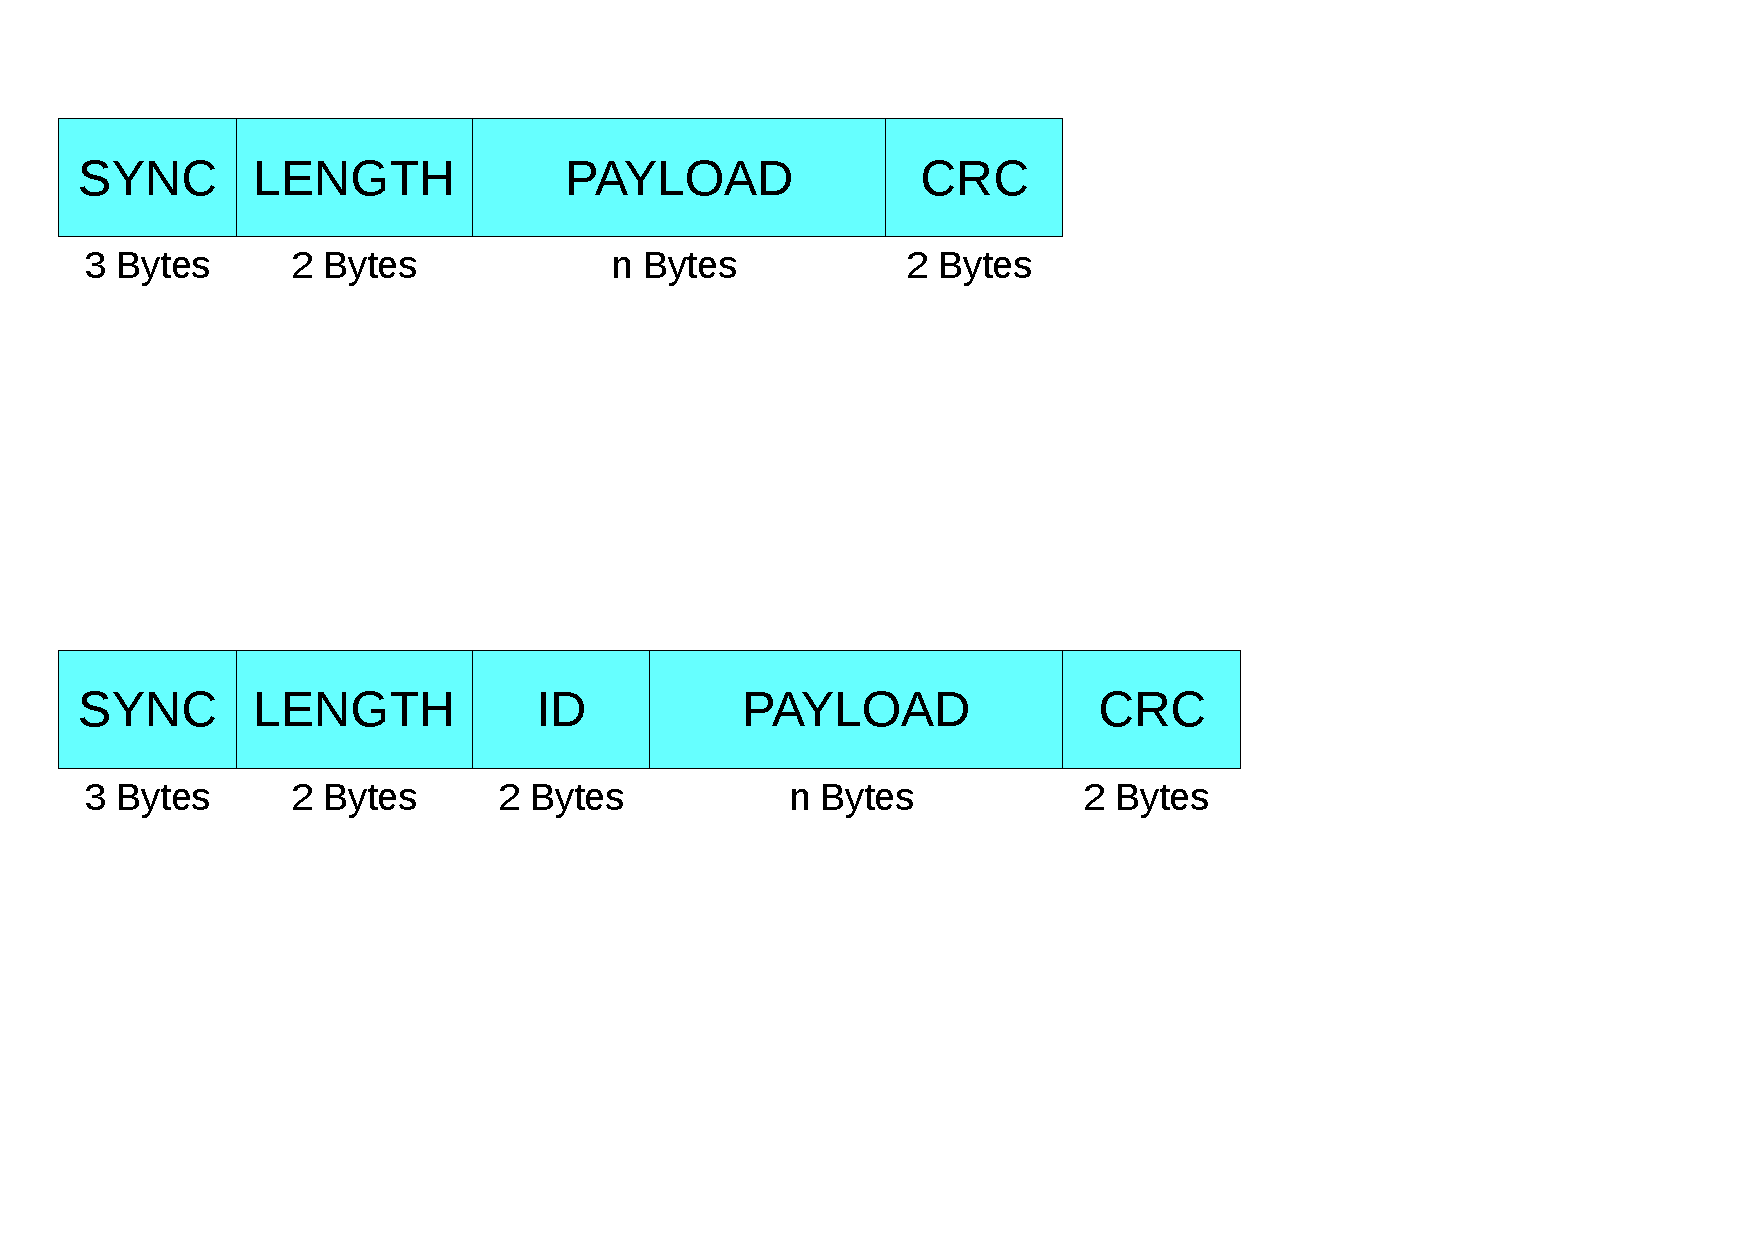
\includegraphics[scale=0.5, trim={0.5cm 16cm 11cm 2cm},clip]{pic/50_app/packet.pdf}
  \caption{Packet Struktur ohne ID}
  \label{fig:packet1}
%		\end{center}
		\end{subfigure}
		
		\begin{subfigure}{0.49\textwidth}
%		\begin{center}
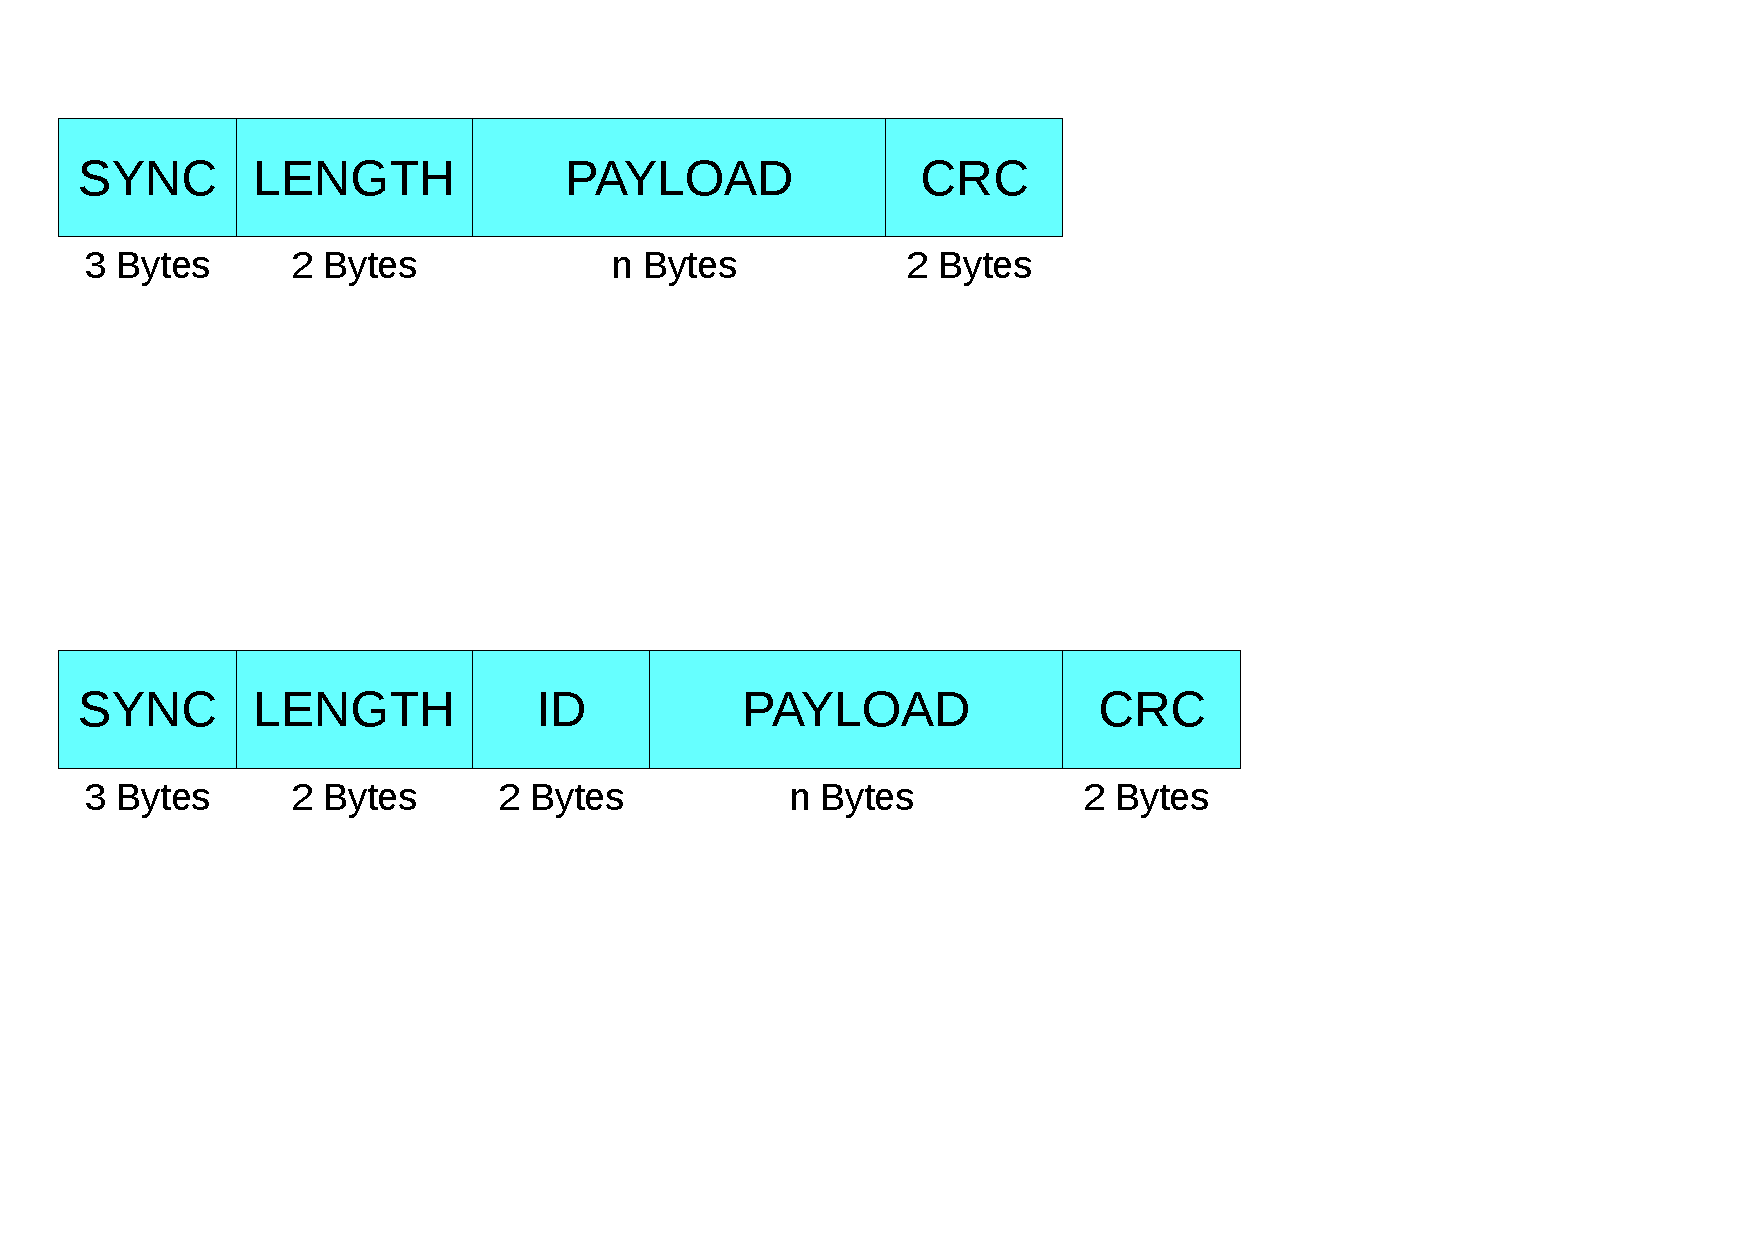
\includegraphics[scale=0.5, trim={0.5cm 7cm 1cm 10.5cm},clip]{pic/50_app/packet.pdf}
  \caption{Packet Struktur mit ID}
  \label{fig:packet2}
%		\end{center}
		\end{subfigure}
		
		\caption{Packetstruktur}
		\label{fig:Packet Struktur}
	\end{center}
\end{figure}


\noindent Die genaue Paketstruktur ist in folgender Tabelle aufgezeigt. Es handelt sich um das 'little Endian' Format. 
\begin{table}[ht]
\begin{center}
  \begin{tabular}{| c | l | c |}
    \hline
    Name & Inhalt & Länge (Byte) \\
    \hline
    SYNC  & Synchronisationszeichen  & 3 \\
          & ASCII: \#:\_                          &  \\
    \hline
    LENGTH & Länge & 2 \\
           & Bytelänge der Payload &  \\
    \hline
    ID & Identifikation: & 2 \\
       & Bit Array, bei welchem jedes Bit einem definierten uORB Topic entspricht.&  \\
    \hline
    PAYLOAD & Nutzdaten & n \\
            & Daten im roh Format & \\
    \hline
    CRC & Checksumme & 2 \\
        & CRC16 über die SYNC, LENGTH, (ID) und PAYLOD Daten & \\
    \hline
  \end{tabular}
  
  \caption{Paketstruktur Beschreibung}
  \label{tab:Paketstruktur Beschreibung}
  
\end{center}
\end{table}

\noindent Durch die ID kann festgelegt werden, welche uORB Topics in der PAYLOAD vorhanden sind. Damit alle Permutation möglich sind, ist jedem ID-Bit ein uORB Topic zugewiesen.

\begin{table}[ht]
\begin{center}
  \begin{tabular}{| l | l |}  
    \hline
    Bits [MSB ... LSB] & uORB Topic Name \\ \hline
    1xxx'xxxx xxxx'xxxx & Heartbeat\\ \hline
    x1xx'xxxx xxxx'xxxx & Sensor combined \\ \hline
    xxxx'xxxx 1xxx'xxxx & Actuator armed \\ \hline
    xxxx'xxxx x1xx'xxxx & Actuator controls \\ \hline
  \end{tabular}  
  \caption{Paket ID}
  \label{tab:Paket ID}  
\end{center}
\end{table}


\clearpage
\noindent Bei den empfangenen Daten muss zuerst der Beginn festgelegt werden. Für dies wird eine Parser (Abbildung \ref{fig:Statemachine Parser} verwendet.


\begin{figure}[ht]
  \begin{center}
  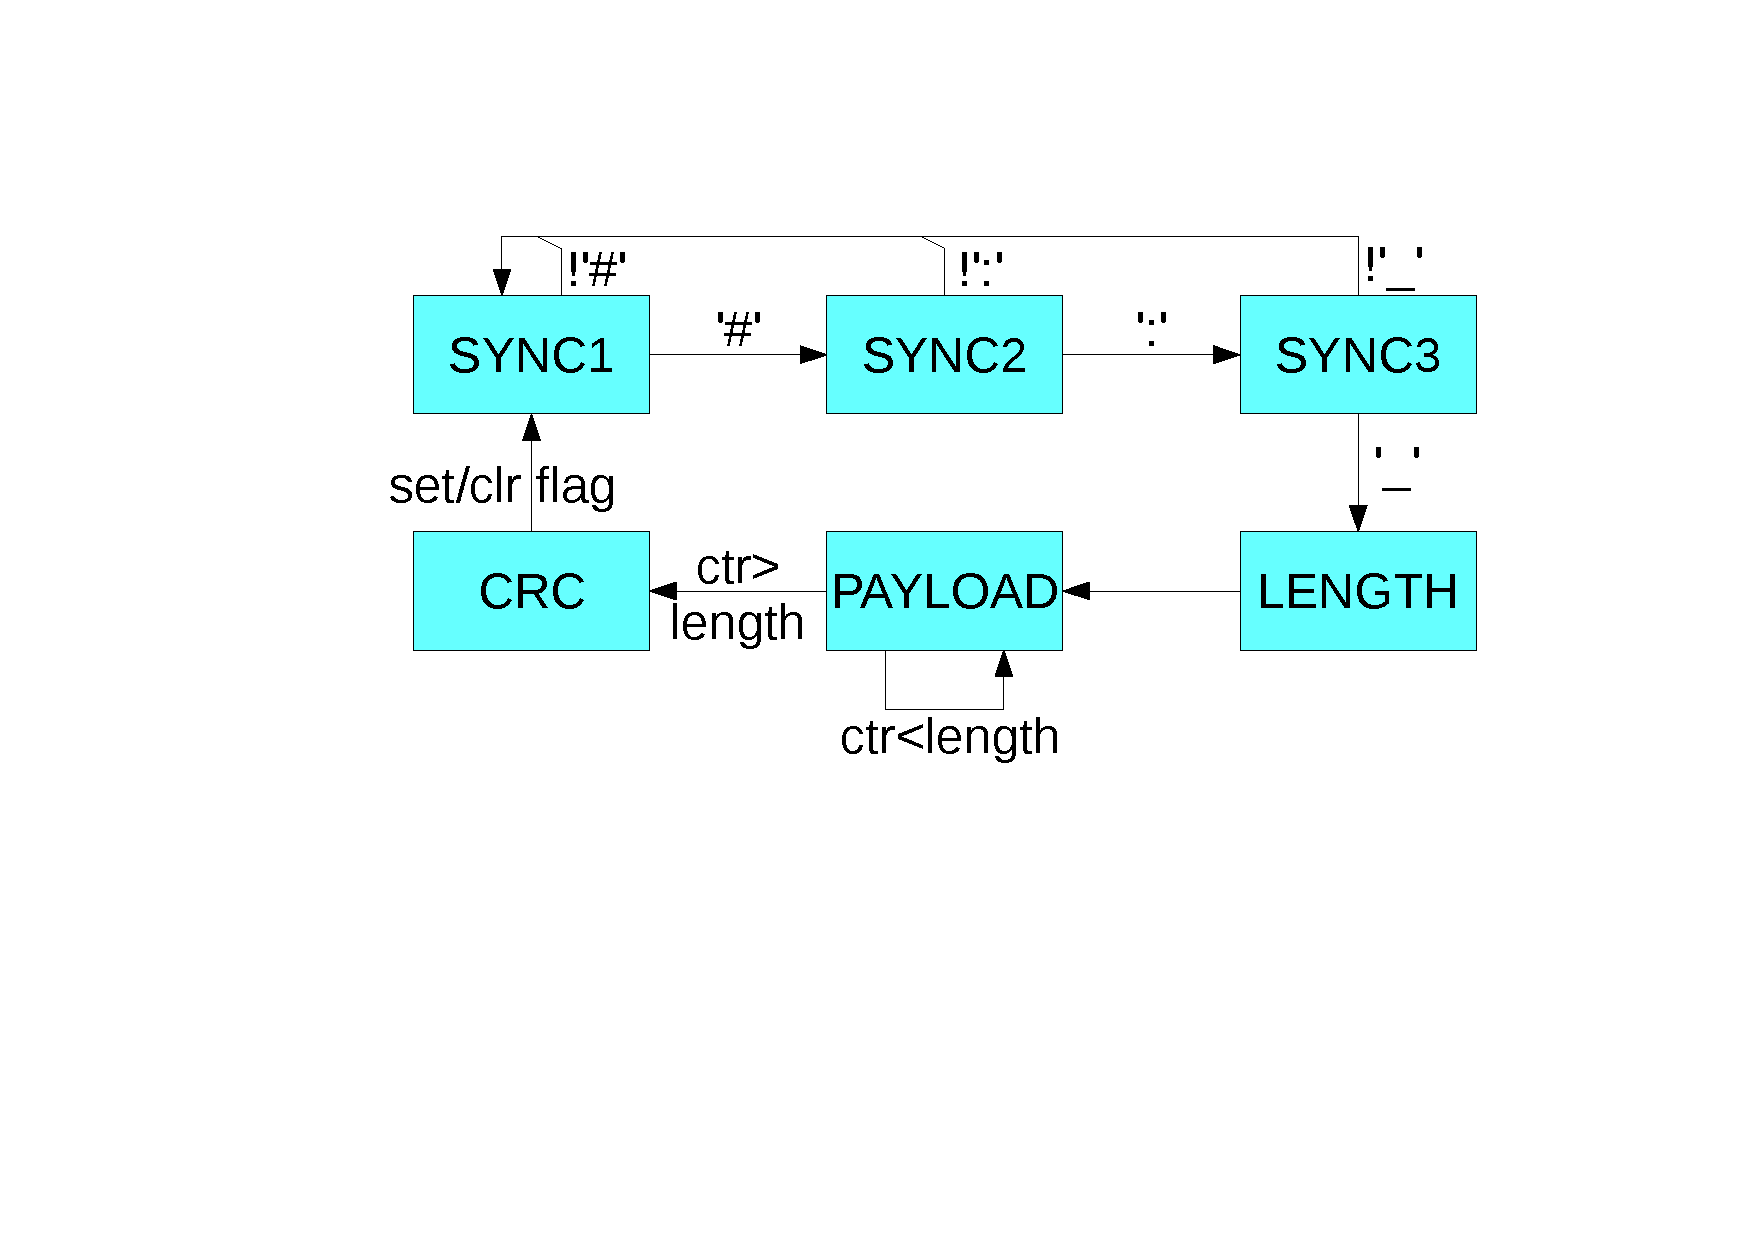
\includegraphics[scale=0.5, trim={6cm 8cm 4cm 4cm},clip]{pic/50_app/statemachine_parser.pdf}
  \caption{Statemachine Parser}
  \label{fig:Statemachine Parser}
  \end{center}
\end{figure}

\noindent Die Synchronisationsreihenfolge \#:\_ wurde desshalb gewählt, da diese eine zufällige Reihenfolge an Bits enthält. Weiter ist die Chance, dass dieses Bit-Reihenfolge erscheint $P = \frac{1}{2^{3\cdot8 Bits}}\approx\frac{1}{16\cdot 10^6} \approx 6 \cdot 10^{-8}$. Weiter sollte diese Reihenfolge im ASCII Format leicht ersichtlich sein, um das Debuggen zu vereinfacht. ASCII Steuerzeichen wurden bewusst nicht verwendet, da diese ja nach Betriebssystem, sowie Programm anders interpretiert werden können. \\
Am Ende des Pakets wird eine CRC16 mit dem Polynom $0x8005 = x^{16} + x^{15} + x^2 + 1$ angehängt. Durch Verwendung von nur einer Checksumme kann der Fehler im Paket nicht lokalisiert und korrigiert werden. Für die HiL Simulation steht die Geschwindigkeit jedoch im Vordergrund. Falls die Checksumme nicht übereinstimmt, wird das gesamte Paket verworfen.

\clearpage

\subsubsection{Serial}
Die serielle Datenübertragung wird per UART realisiert. Das Pixhawk besitzt fünf serielle Interfaces. Einige dieser sind bereits reserviert, z.B. das GPS. Drei Interfaces stehen für die Entwickler zur Verfügung, AMC0 (USB Anschluss), ttyS5 (Serial 4) und ttyS6 (Serial5). Diese Bezeichnungen basieren auf GNU/Linux. Auf AMC0 und ttyS5 sind bereits belegt durch eine nsh. Die Implementation der Lese- und Schreib-Methode sind nicht reentrent. Deshalb sollte die Schnittstelle nur von einem Thread verwendet werden. Aus diesem Grund wurde \textbf{ttyS6} für den Datenstrom verwendet, damit keine anderen App das Interface belegt.\\ 

\noindent Auf der Host Seite wird ein USB $\leftrightarrow$ UART Konverter verwendet. Für diese PAIND Arbeit wurde ein offizielles FTDI Kabel verwendet. Je nach Anschluss (siehe Abbildung \ref{fig:Serielle Schnitstelle} ) wird eine andere Schnittstelle verwendet. Für diese Arbeit wurde ttyS6 belegt.


\begin{figure}[ht]
	\begin{center}
		\begin{subfigure}{0.49\textwidth}
%			\begin{center}
  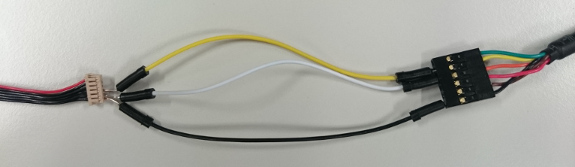
\includegraphics[scale=0.5]{pic/50_app/ttyS5_hw.jpg}
  \caption{ttyS5 mit nsh}
  \label{fig:ttyS5_cable}
%		\end{center}
		\end{subfigure}
		
		\begin{subfigure}{0.49\textwidth}
%		\begin{center}
  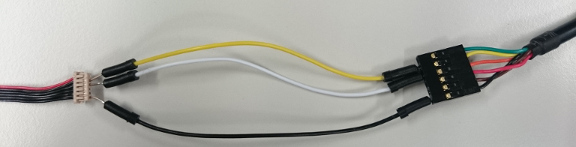
\includegraphics[scale=0.5]{pic/50_app/ttyS6_hw.jpg}
  \caption{ttyS6 ohne nsh}
  \label{fig:ttyS6_cable}
%		\end{center}
		\end{subfigure}
		
		\caption{Serielle Schnitstelle}
		\label{fig:Serielle Schnitstelle}
	\end{center}
\end{figure}


\noindent Anbei die Farbcodierung der Signalleitungen:
\begin{table}[ht]
\begin{center}
  \begin{tabular}{| c | c | c |}
    \hline
    Farbe & Verwendung Pixhawk & Verwendung Host PC \\
    \hline
    gelb  & TX & RX \\
    \hline
    weiss & RX & TX \\
    \hline
    schwarz & GND & GND \\
    \hline
  \end{tabular}
  
  \caption{UART Farbcodierung}
  \label{tab:UART color}
  
\end{center}
\end{table}

\paragraph{Baud}\mbox{}\\
\noindent Das uORB Datenpaket 'Sensor combined' enthält 722 Bytes. Dies könnte eine hohe Bandbreite erfordern. Es ist nicht genau klar, wie oft dieses in der uORB bereitsteht. Deshalb wurde diese Bandbreite gemessen. Dafür wurde die Baudrate sehr hoch angesetzt, damit die Daten sofort gesendet werden und der Buffer kein Überlauf erfährt. Die Messung ergab folgende Werte:
\noindent $\frac{390240 Bytes}{16 s} = 24390 \frac{Byte}{s}$.\\
Jedes Byte enthält zusätzlich ein Start- und Stopbit, somit ergibt sich: \\
$1 \frac{Nutzbyte}{s} = 1 \frac{Startbit}{s} +8 \frac{Nutzbits}{s} +1 \frac{Stopbit}{s} =10 \frac{Bit}{s} = 10 Baud$.\\
Dadurch wird der Umrechnungsfaktor 10 bestummen. Falls nun die gemessen Byterate umgerechnet wird:  $24390 \frac{Byte}{s} = 243900 Baud$.\\

\noindent Die verfügbaren Baud sind [..., 115200, 230400, 460800, 921600]. Damit die Daten keine Verzögerung erfahren und aufgrund bidirektionaler Kommunikation, wurde die Baud von $460800Baud$ gewählt. Bei $921600Baud$ ist die Störungsanfälligkeit noch höher.


\paragraph{Code}\mbox{}\\
Die Implementierung des POSIX Interfaces der seriellen Schnittstelle ist nicht multithread fähig. Dadurch kann nur 1 Thread auf den Filedescriptor zugreifen. Falls ein zweiter Versucht den selben Filedescriptor zu verwenden, kommt es zu Laufzeitfehler.\\

\noindent Die Verwendung des Interfaces ist einfach gehalten.

\begin{lstlisting}
  /** open Serial port **/
  fd_serial = open(PORT_TTYS, O_RDWR);
  if (fd_serial < 0) {
    thread_should_exit = true;
\end{lstlisting}
Durch dieses Kommando wird dem Filedescriptor fd\_serial eine neue Indexnummer zugewiesen. Alle weiteren Aktionen basieren nun auf diesem Index. Falls der Index kleiner 0 ist, konnte der Port nicht geöffnet werden.\\

\begin{lstlisting}
  write(fd_serial, buf_send, i);
\end{lstlisting}
Das Senden erfolgt durch Übergabe eines char Pointers und der Datenlänge. Hierbei ist zu beachten, dass die Länge in Form des Datentyps angegeben wird. i=1 entspricht für ein char Pointer 8 Bits.\\


\begin{lstlisting}
  /** poll-file-descriptor for serial interface **/
  struct pollfd fds_serial[]= {
    {.fd = fd_serial,   .events = POLLIN },};

  [...]

  poll_ret = poll(fds_serial, 1, TIMEOUT_RCV_POLL_MS);
  if (poll_ret > 0){
    //We got new data on serial Interface
  }
\end{lstlisting}
Die uORB kann auch Filedescriptors aufnehmen. Durch obigen Code wird die serielle Schnittstelle per uORB überwacht. Falls neue Daten anliegen oder das Timeout auf Zeile 7 ausgelaufen ist, wird ein Betriebssystem Interrupt ausgeführt. Falls der return Wert grösser 0 ist, liegen neue Daten an der seriellen Schnittstelle.\\


\begin{lstlisting}
  int ctr = read(fd_serial, buf_tmp, BUFFER_SIZE_RCV);
\end{lstlisting}
Das Auslesen der Daten erfolgt ressourcenschonend. Man übergibt der read Funktion den Filedescriptor, die Adresse des char Buffers und die maximale Anzahl Zeichen, welche man empfangen möchte. Als return Wert bekommt man die Anzahl empfangener Daten, welche nun im char Buffer bereitstehen. 

\clearpage

\subsubsection{Auswertung}
Mit dieser App ist eine HiL Simulation auf seitens Pixhawk möglich. Es können die Stellgrössen der Aktuatoren über die UART gesendet werden und generierte Sensorwerte den Reglern "vorgehalten" werden. Die App ist sehr ressourcenschonend mit nur 12\% CPU Auslastung, trotz den grossen Datenmengen. Falls die komplette Bandbreite benützt würde, wäre die CPU Auslastung voraussichtlich ~25\%.


\clearpage

\subsection{Simulink}
\label{sec:Simulink}
Auf Simulink Seite wird die Umgebungssimulation vorgenommen. Dafür müssen die empfangenen Datenpakete auch auf dieser Seite zuerst geparst werden. Anschliessend durchlaufen die Werte einen Algorithmus, welcher neue Werte an das Pixhawk sendet.

\subsubsection{Kommunikation}
Simulink stellt in der 'Instrumental Control Toolbox' TCP/UDP, IP und serielle Kommunikationsblöcke zur Verfügung. Diese Toolbox ist nicht in der HSLU Lizenz einbezogen.\\

\noindent Für die Datenübertragung per Serial Port muss dieser zuerst korrekt konfiguriert werden im Block 'Serial Configuration' (Abbildung \ref{fig:conf_conf}). Die Baud, Kontrollbits, Symbolgrösse, Byte-Reihenfolge sowie ein Timeout müssen angegeben werden.\\

\begin{figure}[H]
  \begin{center}
  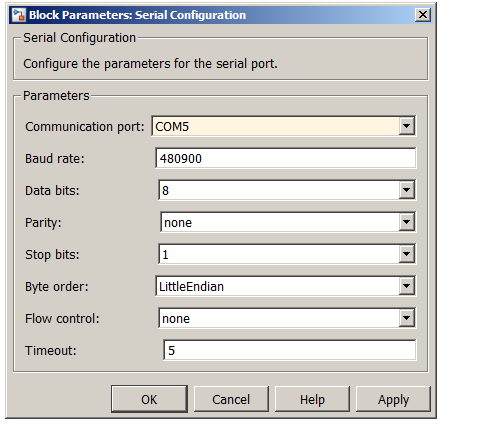
\includegraphics[width=0.5\textwidth]{pic/60_simulink/conf_conf.png}
  \caption{Einstellungen Konfigurationsblock}
  \label{fig:conf_conf}
  \end{center}
\end{figure}


\noindent Der Empfängerblock (Abbildung \ref{fig:conf_rcv}), welcher die Daten ins Simulink einspeist, muss auch konfiguriert werden. Hierbei gilt zu beachten, dass der 'Blocking Mode' ausgeschaltet wird. Dieser Parameter erlaubt, dass die Simulation weiterlaufen kann, obwohl keine neuen Daten empfangen wurden. Der Parser kann auch gleich übergeben werden im Header Feld. In diesem Block wird versucht, alle 50ms ein Packet von 772 Bytes zu empfangen. Diese Paketstruktur entsprechen dem Format von Abbildung \ref{fig:packet1} und muss für die Verwendung zuerst noch geparst werden. Würde man jedes Byte einzeln empfangen, wäre dies sehr ineffizient. Der Block enthält ein Sleep Befehl von 1ms. Dies würde bei einer kurzen Abtastzeit stark ins Gewicht fallen. Bei den 50ms im Projekt ist dies jedoch vernachlässige.\\

\begin{figure}[H]
  \begin{center}
  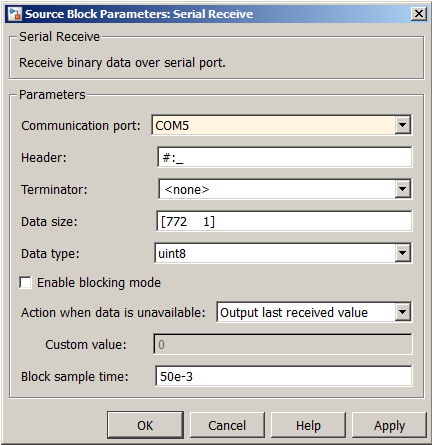
\includegraphics[width=0.5\textwidth]{pic/60_simulink/conf_rcv.png}
  \caption{Einstellungen Empfänger Block}
  \label{fig:conf_rcv}
  \end{center}
\end{figure}

\noindent Der Sendeblock (Abbildung \ref{fig:conf_send}) extrahiert die  Simulationsdaten und sendet diese ans Pixhawk. Die drei Synchronisationsbyte können als Paketkopf übergeben werden.

\noindent
\begin{figure}[H]
  \begin{center}
  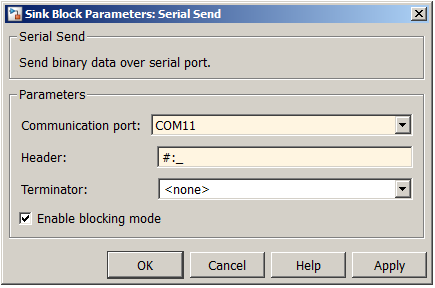
\includegraphics[width=0.5\textwidth]{pic/60_simulink/conf_send.png}
  \caption{Einstellungen Sender Block}
  \label{fig:conf_send}
  \end{center}
\end{figure}

\noindent Diese drei Blöcke übernehmen die gesamte Kommunikation auf Seite Simulink. Der Inhalt des Datenpakets müssen nun gegliedert  und einer Typenumwandlung unterzogen werden.

\clearpage
\subsubsection{Parser}
Damit die Daten im Simulink in sinnvoller Struktur verfügbar sind, muss der Inhalt entpackt werden. Dazu ist momentan die Struktur der Daten nötig. Falls die Paket ID implementiert wäre, könnte man anhand der gesetzten ID-Bits diese entpacken. Diese Aufgabe übernimmt ein 'Interpreted MATLAB Function' Block. 


\begin{lstlisting}
function output_args = parser_small(input_args)

global pck_length;

% Parse package length
pck_length = input_args(1,:);
pck_length = pck_length + 256*input_args(2,:);

% Parse package ID


% Parse package payload and convert
time = double(typecast(uint8(input_args(3:10)), 'uint64'))/1e6;
g_x = double(typecast(uint8(input_args(207:210)), 'single'));
g_y = double(typecast(uint8(input_args(211:214)), 'single'));
g_z = double(typecast(uint8(input_args(215:218)), 'single'));    

% crc detector


% output data
output_args = [time ; g_x ; g_y ; g_z ];            
\end{lstlisting}
\medskip

\noindent Der Parser muss folgende Aufgaben übernehmen:
\begin{table}[ht]
\begin{center}
  \begin{tabular}{| l | l | }
    \hline
    Zeile & Aktion \\
    \hline
    6...7  & Paketlänge zusammensetzten \\
    \hline
    10  & ID auslesen \\
    \hline
    13..16  & Nutzdaten auslesen und casten \\
    \hline
    19  & CRC16 Überprüfung der Nutzdaten \\
    \hline 
    22  & Vektorausgabe der Werte \\
    \hline 
  \end{tabular}
  
  \caption{Simulink Parser}
  \label{tab:Simulink Parser}
  
\end{center}
\end{table}



%\begin{figure}[ht]
%  \begin{center}
%  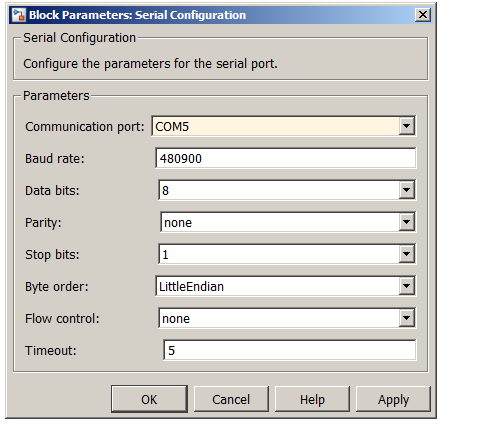
\includegraphics[width=0.5\textwidth]{pic/60_simulink/conf_conf.png}
%  \caption{tmp}
%  \label{fig:temp}
%  \end{center}
%\end{figure}


\clearpage

\subsection{Simulation}
Durch Verwendung der Pixhawk App sowie der Simulink Blöcke kann eine einfache Datenstromverarbeitung erfolgen. Die digitalen Dateien sind im Kapitel \ref{sec:Anhang} vorhanden.\\

\noindent
Das Subsystem in Abbildung \ref{fig:sub_sim_system} konfiguriert den COM Port und öffnet diesen. Falls dies fehlschlägt wird die Simulation automatisch abgebrochen.
\begin{figure}[H]
  \begin{center}
  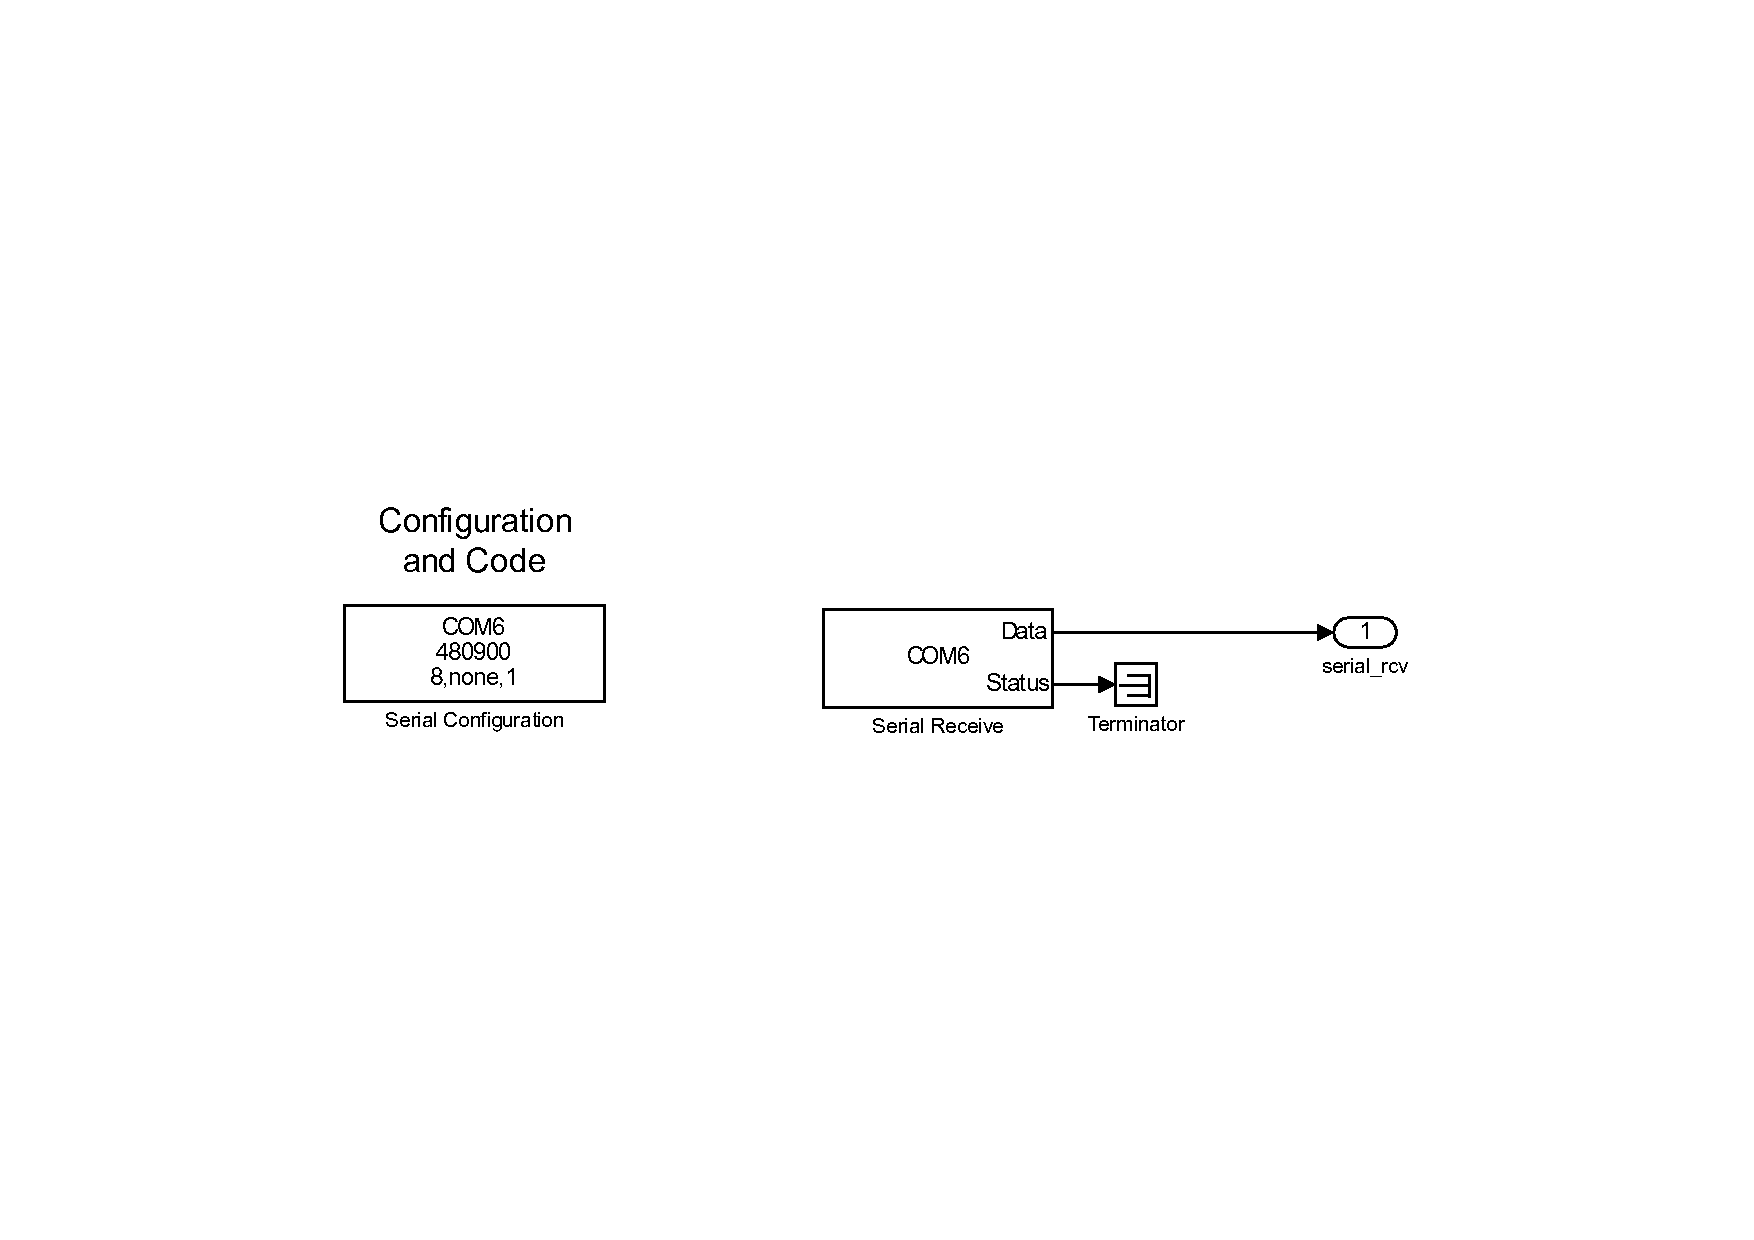
\includegraphics[scale=0.6, trim={5cm 8.5cm 5.5cm 8.5cm},clip]{pic/70_eigene_app/Serial_output.pdf}
  \caption{Serielle Schnittstelle}
  \label{fig:sub_sim_system}
  \end{center}
\end{figure}

\noindent
Die Pakete werden im System verarbeitet. Dazu wird eine 'Interpreted MATLAB Function' verwendet. Dieser Block unterstützt nur das double Format. Aus diesem Grund wurde ein Datentyp Konverter hinzugefügt. Der Parser liefert ein Vektor, welcher mit einem Demultiplexer die Kanäle separiert.
 \begin{figure}[ht]
  \begin{center}
  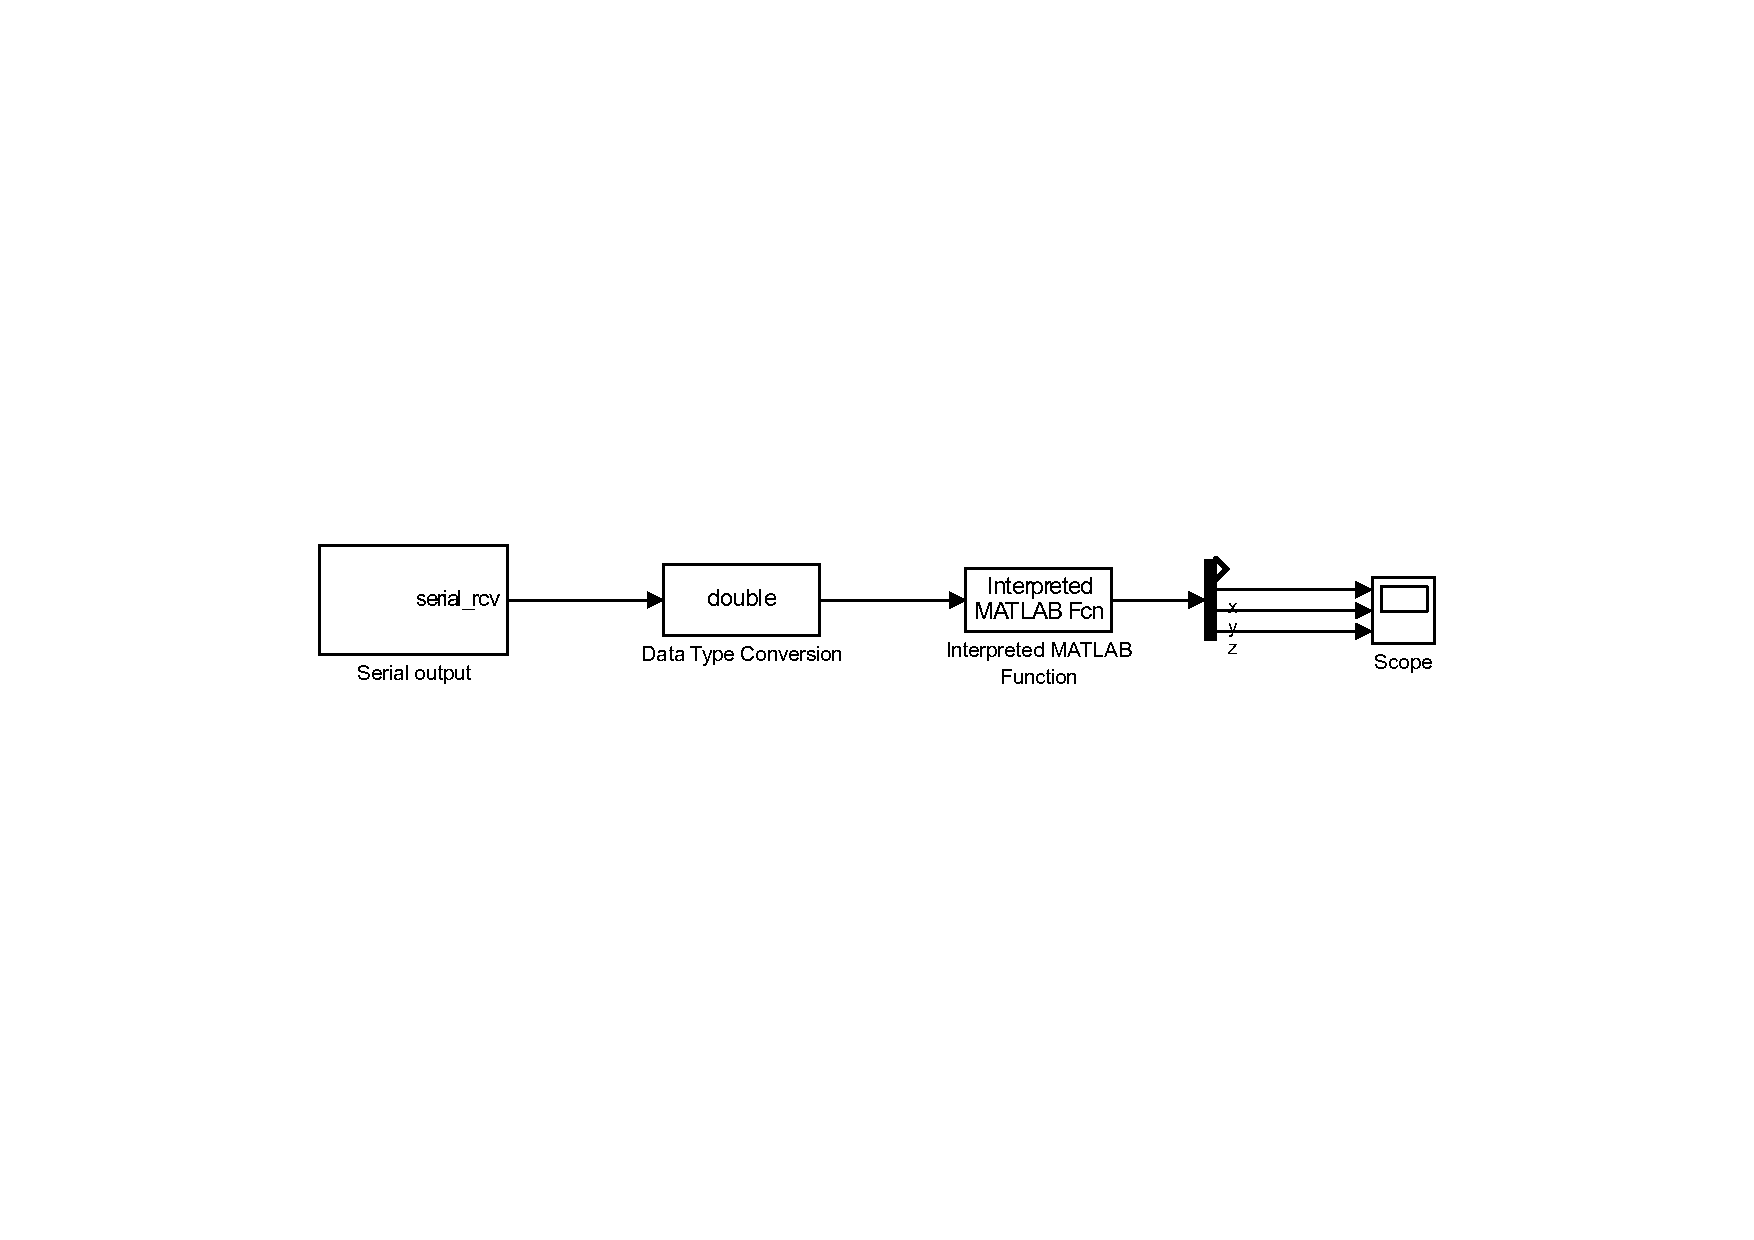
\includegraphics[scale=0.6, trim={5cm 9cm 4.8cm 8.5cm},clip]{pic/70_eigene_app/sys_main.pdf}
  \caption{Serielle Schnittstelle}
  \label{fig:main_sim_system}
  \end{center}
\end{figure}

\noindent
In der Abbildung \ref{fig:accel_looping} ist der Scope ersichtlich. Auf der x-Achse befindet sich die Zeit in Sekunden. Die y-Achse beschreibt die Beschleunigung in x, y und z-Richtung in $\frac{m}{s^2}$.  Der Scope kann während der Simulation geöffnet werden und zeigt die Daten zur Laufzeit an.
\begin{figure}[ht]
  \begin{center}
  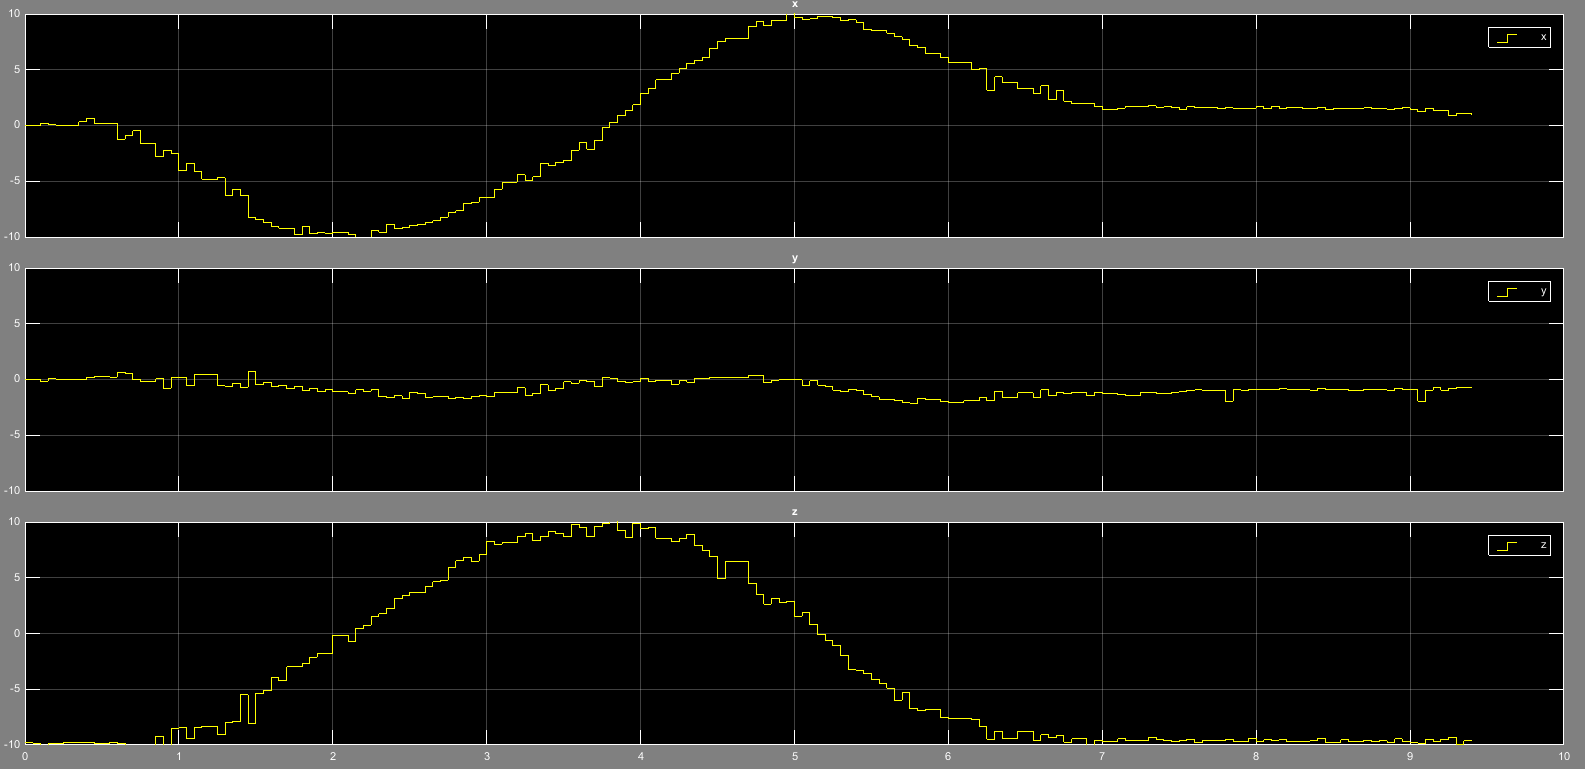
\includegraphics[scale=0.3]{pic/70_eigene_app/looping.png}
  \caption{Accelorometer während eines Looping}
  \label{fig:accel_looping}
  \end{center}
\end{figure}






\clearpage


\section{Auswertung}

\subsection*{Fachliches Fazit}
\noindent 
Durch die Pixhawk App wurde ein mächtiges Tool entwickelt, um Daten auszulesen, zu modifizieren und einzuspeisen. Dieses kann auch als Basis für andere Aufgaben dienen. Selbes gilt auch für die Simulink Blöcke. \\
\noindent
Durch das Zusammenspiel der Pixhawk App sowie dem Simulinkmodell wurde erfolgreich eine stabile Datenstromverarbeitung realisiert. Die Daten können auf der jeweiligen Seite mit einer hohen Baud gesendet, empfangen und interpretiert werden. Die CPU Auslastung ist auf beiden Seiten sehr gering in Anbetracht der grossen Datenmengen.\\
Eine HiL Simulation konnte in der vorgegebenen Zeit nicht realisiert werden.

\subsection*{Persönliches Fazit}
Durch dieses spannende Arbeit erhielt ich Einblicke in die Aviatik, Flugregelung, C sowie C++ Programmierung
Die Arbeit war in drei Aufgaben aufgeteilt und jede Arbeit erforderte unterschiedliche Tools. Zum einen musste man sich in das PSP und den Code Composer einarbeiten, zu anderen in die Pixhawk Firmware und zum Schluss noch ins Simulink mit einer Datenstrom-Verarbeitung und -Ausgabe. Jedes dieser Tools benötigte eine Einarbeitungszeit. Das erlernte Hochschul-Wissen konnte teilweise angewendet werden, jedoch haben Elektroniker ein sehr kleines Programmierwissen im Vergleich zu den Informatikern. Aus meiner Sicht hätte ein Interdisziplinäres Team zu einem besseren Ergebnis geführt.\\
Durch die Einzelarbeit konnte ich jedoch einen grösseren, persönlichen Nutzen erarbeiten. Es ermöglichte einen Einblick in die anderen Fachgebiete.

\clearpage



%Bibliography

%\section{Quellenverzeichnis}
%\nocite{*}
%\bibliography{tex/80_bib/bibliographie}
%\clearpage


%Anhang
\section{Anhang}
\label{sec:Anhang}
\appendix

\nocite{*}
  \bibliography{tex/80_bib/bibliographie}
  \clearpage
\listoffigures
\addcontentsline{toc}{section}{\listfigurename}
\medskip

\listoftables
\addcontentsline{toc}{section}{\listtablename}


\clearpage 
\section{CD ROM}

\clearpage
\section{Code Pixhawk}

\subsection*{my\_app.h}
\lstinputlisting[language=c]{src/my_app/my_app.h}
%\lstinputlisting[firstline=37, lastline=45]{src/my_app/my_app.h}

\subsection*{my\_app.c}
\lstinputlisting[language=c]{src/my_app/my_app.c}

\subsection*{crc.h}
\lstinputlisting{src/my_app/crc.h}

\subsection*{crc.c}
\lstinputlisting{src/my_app/crc.c}

\subsection*{CMakeLists.txt}
\lstinputlisting[firstline=35, lastline=49]{src/my_app/CMakeLists.txt}



\section{Code Simulink}

\subsection*{script.m}
\lstinputlisting{src/simulink/script.m}

\subsection*{parser\_small.m}
\lstinputlisting{src/simulink/parser_small.m}


\clearpage
\section{Aufgabenstellung}

Die Aufgabenstellung enthält 5 Punkt, a bis e. \\

\begin{table}[ht]
\begin{tabular}{c | cl}
\hline

Punkt & \multicolumn{2}{l}{ Aufgaben}\\
\hline

a & $\cdot$ & Einarbeitung in die Pixhawk Firmware\\
  & $\cdot$ & Die Programmiertechniken, Designpatterns sollen vertsanden werden\\
  & $\cdot$ & Eigene Test-App mit Datenstomverarbeitung erstellen\\
  & $\cdot$ & Eigene Test-App mit Datenstomverarbeitung demonstrieren\\
\hline

b & $\cdot$ & In Simulink soll eine Übersicht an Möglichkeiten erstellt werden \\
  & & um mit dem Pixhawk-Modul zu kommunizieren, dass die \\
  & & Hardware-in-the-loop Simulation verwirklicht werden kann\\
\hline

c & $\cdot$ & Pixhawk Firmware erweitern, dass die Anbindung an Simulink \\
  & & durch starten einer einzelnen App möglich wird\\
\hline

d & $\cdot$ & Eine einfache Hardware-in-the-loop Simulation soll auf Seite \\
  & & Simulink programmiert werden\\
  & $\cdot$ & Die Simulation muss demonstriert werden\\
\hline

e & & Optional:\\
  & $\cdot$ & Programmieren verschiedener Tests\\
  & $\cdot$ & Einzelne Testcases in Testscenarien zusammenfassen\\
  & $\cdot$ & Automatisierte Ablauf von Testscenarien soll erfolgen\\
\hline
\end{tabular}

\label{tab:aufgaben}
\caption{Aufgaben}
\end{table}


\medskip

\noindent Die Punkte a bis d müssen vor dem Abschlusstermin erfüllt sein.\\


\clearpage
\section{Projektplan}

Meilenstein a: 26.10.2015 bis 20.11.2015\\
Meilenstein b: 26.10.2015 bis 20.11.2015\\
Die Meilensteine werden in Form einer kurzen Präsentation abgehalten.\\\\

\noindent Abgabe Schlussbericht: 18.12.2015, 16:00 im Raum D311\\
Abschlusspräsentation: Zwischen 14.12.2015 bis 22.01.2016


\clearpage

\begin{landscape}
\subsection*{Projektplan}
\includegraphics[scale=0.75,page=2]{tex/90_appendix/schedule.pdf} 
\clearpage
\includegraphics[scale=0.75,page=3]{tex/90_appendix/schedule.pdf} 
\clearpage
\includegraphics[scale=0.75,page=5]{tex/90_appendix/schedule.pdf} 
\end{landscape}


\end{document}